%
%   Prof. Dr. Julian Reichwald
%   auf Basis einer Vorlage von Prof. Dr. Jörg Baumgart
%   DHBW Mannheim
%
%
%	ACHTUNG: Für das Erstellen des Literaturverzeichnisses wird das modernere Paket biblatex
%			 in Kombination mit biber verwendet -- nicht mehr das ältere BibTex!
% 			 Bitte stellen Sie ggf. Ihre TeX-Umgebung entsprechend ein
% 			 (z.B. TeXStudio: Einstellungen --> Erzeugen --> Standard Bibliographieprogramm: biber)
%

\documentclass[
	12pt,
	BCOR=5mm,
	DIV=12,
	headinclude=on,
	footinclude=off,
	parskip=half,
	bibliography=totoc,
	listof=entryprefix,
	toc=listof,
	pointlessnumbers,
	plainfootsepline]{scrreprt}

%	Konfigurationsdatei einziehen
% !TEX root =  master.tex
% 		HYPERREF
%
\usepackage[
	hidelinks=true % keine roten Markierungen bei Links
]{hyperref}

% Zwei eigene Befehle zum Setzen von Autor und Titel. Ausserdem werden die PDF-Informationen richtig gesetzt.
\newcommand{\TitelDerArbeit}[1]{\def\DerTitelDerArbeit{#1}\hypersetup{pdftitle={#1}}}
\newcommand{\AutorDerArbeit}[1]{\def\DerAutorDerArbeit{#1}\hypersetup{pdfauthor={#1}}}
\newcommand{\Firma}[1]{\def\DerNameDerFirma{#1}}
\newcommand{\Kurs}[1]{\def\DieKursbezeichnung{#1}}

\usepackage{tocbibind}  % DANIEL fügt das Inhaltsverzeichnis zum Inhaltsverzeichnis hinzu  // ursprünglich nicht vorhanden

\usepackage{footnote}  % DANIEL hinzugefügt

%		FONT AND INPUT ENCODING
%
\usepackage[T1]{fontenc}
\usepackage[utf8]{inputenc}

%		CALCULATIONS
%
\usepackage{calc} % Used for extra space below footsepline

%		LANGUAGE SETTINGS
%
\usepackage[ngerman]{babel} 	% German language
\usepackage[german=quotes]{csquotes} 	% correct quotes using \enquote{}

%\usepackage[english]{babel}   % For english language
%\usepackage{csquotes} 	% Richtiges Setzen der Anführungszeichen mit \enquote{}


%		BIBLIOGRAPHY SETTINGS
%
 \usepackage[backend=biber, autocite=footnote, style=authoryear, dashed=false]{biblatex} 	%Use Author-Year-Cites with footnotes
% \usepackage[backend=biber, autocite=inline, style=ieee]{biblatex} 	% Use IEEE-Style (e.g. [1])
% \usepackage[backend=biber, autocite=inline, style=alphabetic]{biblatex} 	% Use alphabetic style (e.g. [TGK12])

%%%% APA/Harvard-Style (bitte die nächten zwei Zeilen auskommentieren)
%\usepackage[backend=biber, style=apa]{biblatex} 	
%\DeclareLanguageMapping{german}{german-apa}

\DefineBibliographyStrings{ngerman}{  %Change u.a. to et al. (german only!)
	andothers = {{et\,al\adddot}},
}

%%% Uncomment the following lines to support hard URL breaks in bibliography 
\apptocmd{\UrlBreaks}{\do\f\do\m}{}{}
\setcounter{biburllcpenalty}{9000}% Kleinbuchstaben
\setcounter{biburlucpenalty}{9000}% Großbuchstaben


\setlength{\bibparsep}{\parskip}		%add some space between biblatex entries in the bibliography
\addbibresource{bibliography.bib}	%Add file bibliography.bib as biblatex resource


%		FOOTNOTES 
%
% Count footnotes over chapters
\usepackage{chngcntr}
\counterwithout{footnote}{chapter}

%     	ACRONYMS
%%%
%%% WICHTIG: Installieren Sie das neueste Acronyms-Paket!!!
%%%
\makeatletter
\usepackage[printonlyused]{acronym} % nur verwendete werden angezeigt
%\usepackage{acronym} % alle werden angezeigt
\@ifpackagelater{acronym}{2015/03/20}
  {%
    \renewcommand*{\aclabelfont}[1]{\textbf{\textsf{\acsfont{#1}}}}
  }%
  {%
  }%
\makeatother

%		LISTINGS
\usepackage{listings}	%Format Listings properly
\renewcommand{\lstlistingname}{Quelltext} 
\renewcommand{\lstlistlistingname}{Quelltextverzeichnis}
\lstset{numbers=left,
	numberstyle=\tiny,
	captionpos=b,
	basicstyle=\ttfamily\small}


%		EXTRA PACKAGES
\usepackage{lipsum}    %Blindtext
\usepackage{graphicx} % use various graphics formats
\usepackage[german]{varioref} 	% nicer references \vref
\usepackage{caption}	%better Captions
\usepackage{booktabs} %nicer Tabs
\usepackage{array}
\usepackage{eurosym} %Eurosymbol
%\newcolumntype{P}[1]{>{\raggedright\arraybackslash}p{#1}}


%		ALGORITHMS
\usepackage{algorithm}
\usepackage{algpseudocode}
\renewcommand{\listalgorithmname}{Algorithmenverzeichnis }
\floatname{algorithm}{Algorithmus}


%		FONT SELECTION: Entweder Latin Modern oder Times / Helvetica
\usepackage{lmodern} %Latin modern font
%\usepackage{mathptmx}  %Helvetica / Times New Roman fonts (2 lines)
%\usepackage[scaled=.92]{helvet} %Helvetica / Times New Roman fonts (2 lines)

%		PAGE HEADER / FOOTER
%	    Warning: There are some redefinitions throughout the master.tex-file!  DON'T CHANGE THESE REDEFINITIONS!
\RequirePackage[automark,headsepline,footsepline]{scrpage2}
\pagestyle{scrheadings}
\renewcommand*{\pnumfont}{\upshape\sffamily}
\renewcommand*{\headfont}{\upshape\sffamily}
\renewcommand*{\footfont}{\upshape\sffamily}
\renewcommand{\chaptermarkformat}{}

\clearscrheadfoot

\ifoot[\rule{0pt}{\ht\strutbox+\dp\strutbox}DHBW Mannheim]{\rule{0pt}{\ht\strutbox+\dp\strutbox}DHBW Mannheim}
\ofoot[\rule{0pt}{\ht\strutbox+\dp\strutbox}\pagemark]{\rule{0pt}{\ht\strutbox+\dp\strutbox}\pagemark}

\ohead{\headmark}


\begin{document}

%% BITTE GEBEN SIE HIER DEN TITEL UND DIE AUTORIN / DEN AUTOR DER ARBEIT AN!
%% DIESE INFORMATIONEN _MÜSSEN_ GESETZT SEIN, UM TITELBLATT, ABSTRACT UND 
%% EIGENSTÄNDIGKEITSERKLÄRUNG AUTOMATISCH ANZUPASSEN!
\TitelDerArbeit{Unternehmenssimulationsspiel Baubranche}
\AutorDerArbeit{Daniel Pies}
\Firma{SV Informatik GmbH}
\Kurs{WWI 16 SEA}

\pagenumbering{roman} % Römische Seitennummerierung

\begin{titlepage}
\begin{minipage}{\textwidth}
		\vspace{-2cm}
		\noindent 
\includegraphics[scale=0.15]{img/firmenlogo.jpg} 
		\hfill   
\includegraphics{img/logo.jpg}
\end{minipage}
\vspace{1em}
\sffamily
\begin{center}
	\textsf{\large{}Duale Hochschule Baden-W\"urttemberg\\[1.5mm] Mannheim}\\[4em]
	\textsf{\textbf{\Large{}Fallstudie}}\\[3mm]
	\textsf{\textbf{\Large{}\DerTitelDerArbeit}} \\[3cm]
	\textsf{\textbf{\Large{}Studiengang Wirtschaftsinformatik}\\[3mm] \textsf{Studienrichtung Software Engineering}}	
	\vspace{3em}	
%	\textsf{\Large{Sperrvermerk}}
	\vfill

\begin{minipage}{\textwidth}

\begin{tabbing}
	Verfasser: \hspace{0.85cm} \= Manuel Techert \hspace{0.85cm} \= \kill
	Fach: 		\> Fallstudie      \> \\[1.5mm]
	Dozent:		\> Gregor Tielsch  \> \\[3mm]
	Verfasser:  \> Daniel Pies     \> Matrikelnummer: 7104609\\[1.5mm]
				\> Nico Popiolek   \> Matrikelnummer: 9054458\\[1.5mm]
				\> Fabian Pulch    \> Matrikelnummer: 3104428\\[1.5mm]
				\> Manuel Techert  \> Matrikelnummer: 7615798\\[3mm]
	Kurs:		\> WWI 16 SEA      \> \\


\end{tabbing}

\end{minipage}

\end{center}

\end{titlepage} % ursprünglich vor der römischen Seitennummerierung

\normalfont

%--------------------------------
% Verzeichnisse - nicht benötige Verzeichnisse bitte auskommentieren / löschen.
%--------------------------------

\renewcommand{\baselinestretch}{1.15}\normalsize % um Zeilenabstand im Dokument zu ändern

%   Sperrvermerk
% \chapter*{Sperrvermerk}
\addcontentsline{toc}{chapter}{Sperrvermerk}  % DANIEL ursprünglich nicht im Inhaltsverzeichnis
Der Inhalt dieser Arbeit darf weder als Ganzes noch in Auszügen Personen außerhalb des Prüfungsprozesses und des Evaluationsverfahrens zugänglich gemacht werden, sofern keine anders lautende Genehmigung der Ausbildungsstätte vorliegt. 
\cleardoublepage


%	Kurzfassung
%\input{abstract}

%	Inhaltsverzeichnis
\tableofcontents

%	Abbildungsverzeichnis
\listoffigures

%	Tabellenverzeichnis
%\listoftables

%	Listingsverzeichnis
\lstlistoflistings

% 	Algorithmenverzeichnis
% \listofalgorithms

% 	Abkürzungsverzeichnis (siehe Datei acronyms.tex!)
%\clearpage
\chapter*{Abkürzungsverzeichnis}	
\addcontentsline{toc}{chapter}{Abkürzungsverzeichnis}


\begin{acronym}[XXXXX]  % Anzahl der Plätze für Länge der Stellen

%	\acro{DHBW}{Duale Hochschule Baden-Württemberg}



	\acro{ASB}{Anforderungssteckbrief}
	\acro{IDE}{Integrated development environment}
	\acro{IT}{Informationstechnik}
	\acro{JDK}{Java Development Kit}
	\acro{JRE}{Java Runtime Environment}
	\acro{SL}{SonarLint}
	\acro{SQ}{SonarQube}
	\acro{SV}{SV SparkassenVersicherung AG}
	\acro{SVI}{SV Informatik GmbH}
	\acro{SVIS}{Sparkassen Versicherung Informations System}
	\acro{SVS}{Sparkassen-Versicherung Sachsen Holding AG}
	

	
\end{acronym}


%--------------------------------
% Start des Textteils der Arbeit
%--------------------------------
\clearpage
\ihead{\chaptername~\thechapter} % Neue Header-Definition
\pagenumbering{arabic}  % Arabische Seitenzahlen


%	Anleitungs-Datei anleitung.tex einziehen. Auf diese Weise sollten Sie versuchen, für jedes einzelne
% Kapitel eine eigene Datei anzulegen und mittels input-Kommando einzuziehen.
%% !TEX root =  master.tex
\chapter{Gebrauchsanleitung}

\section{Übersicht über die Vorlage}
Die Vorlage wurde im UTF-8 Encoding erstellt. Sollten daher z.\,B. Umlaute in Ihrem \LaTeX-Editor nicht korrekt dargestellt werden, überprüfen Sie bitte die Encoding-Einstellungen des Editors. In seltenen Fällen müssen Sie die Vorlage danach noch einmal neu in den Editor einbinden. 
Die Vorlage beinhaltet die folgenden, in Tabelle \vref{tab:dateien} aufgelisteten Dateien: 
\begin{table}[h!]
	\centering
\begin{tabular}{lp{10cm}}
	\textbf{Dateiname} & \textbf{Beschreibung}\\\toprule
	\texttt{master.tex} & Die Hauptdatei. Alle anderen Dateien werden von dieser Datei eingezogen. \\
	\texttt{abstract.tex} & Die Kurzfassung der Arbeit. \\	
	\texttt{config.tex} & Konfigurationseinstellungen 	 der einzelnen Pakete\\
	\texttt{acronyms.tex} & Definition von Abkürzungen. \\
	\texttt{titlepage.tex} & Titelseite der Arbeit. \textbf{Bitte Anpassen!}\\
	\texttt{anleitung.tex} & Diese Anleitung\\ 
	\texttt{bibliography.bib}&  Die Literaturdatenbank -- hier können Sie die verwendete Literatur einpflegen.\\
	\texttt{ewerkl.tex} & Ehrenwörtliche Erklärung. \textbf{Bitte Anpassen!}\\
	\texttt{appendix.tex} & Anhang bzw. Anhänge \\\bottomrule
\end{tabular}
\caption{\label{tab:dateien}Übersicht über die Dateien der Vorlage}
\end{table}

Es werden -- unter anderem -- die folgenden Zusatzpakete von dieser Vorlage eingezogen und sollten daher in aktuellen Versionen installiert sein: 
\begin{itemize}
	\item\texttt{KOMA-Script} bzw. die Dokumentenklasse \texttt{scrreprt}
	\item\texttt{hyperref} für PDF-Informationen und Links 
	\item \texttt{babel} für länderspezifische Einstellungen
	\item \texttt{csquotes} für sprachabhängige Anführungszeichen (Befehl: \texttt{\textbackslash enquote})
	\item \texttt{acronym} für das Erstellen des Abkürzungsverzeichnisses 
	\item \texttt{booktabs} für das typografisch schöne Setzen von Tabellen 
	\item \texttt{varioref} für einfaches Referenzieren 
	\item \texttt{listings} für schöne Quelltexte
	\item \texttt{algorithm} für schöne Algorithmen
	\item \texttt{bibltatex} und \texttt{biber} für die Erstellung des Literaturverzeichnisses.
\end{itemize}
Alle Konfigurationen dieser Vorlage können in der Datei \texttt{config.tex} eingesehen und ggf. verändert werden. Bitte schauen Sie sich die entsprechenden Dokumentationen 
der Pakete an (\url{https://www.ctan.org}), um deren Verwendung und Möglichkeiten jenseits der hier gezeigten Beispiele zu erlernen.


\section{Übersetzung von \LaTeX-Dateien}
Die Übersetzung von \LaTeX-Dateien erfolgt in mehreren Schritten und unter der Zuhilfenahme unterschiedlicher Programme. Das Hauptdokument (hier die Datei \texttt{master.tex}) wird mittels \texttt{pdflatex} zu einem PDF übersetzt. Ggf. ist eine mehrfache Übersetzung notwendig, um z.\,B. das Inhaltsverzeichnis korrekt darzustellen. 

Für die Einbindung des Literaturverzeichnisses wird nicht mehr das ältere \texttt{bibtex}, sondern das neuere \texttt{biber} in Kombination mit \texttt{biblatex} verwendet. Bitte stellen Sie Ihren \LaTeX-Editor so ein, dass die Verwendung von Biber beim Übersetzungsprozess erfolgt. 

\section{Verwendung von Akronymen}
Akronyme müssen in der Datei \texttt{acronyms.tex} definiert werden (schauen Sie sich hierzu bitte die entsprechende Paket-Dokumentation an!)
Ein definiertes Akronym kann dann mit dem Befehl \texttt{\textbackslash ac} verwenden, so wird z.\,B. \texttt{\textbackslash ac\{DHBW\}} zu \ac{DHBW}. Im weiteren Verlauf wird das 
Acronym dann nur noch in der Kurzform dargestellt: \ac{DHBW}. Die Aufnahme eines verwendeten Akronyms in das Abkürzungsverzeichnis erfolgt automatisch.

\section{Zitieren von Quellen}
Mit dem Befehl \texttt{\textbackslash autocite} kann zitiert werden, z.\,B. so \autocite[Vgl.][S. 18ff.]{ME12}. Sollen mehrere Referenzen auf einmal gesetzt werden, können Sie dies mit dem Befehl \texttt{\textbackslash autocites} erreichen, z.\,B. so\autocites[Vgl.][S. 10]{ME12}[][S. 100]{TD15}. Wird \texttt{autocite} konsequent verwendet, kann in der Datei \texttt{config.tex} der Zitationsstil umgeschaltet werden, ohne dass im Text Veränderungen vorgenommen werden müssen. Vorkonfigurierte Stile sind Alphabetic, Harvard, Fußnotenzitat und IEEE-Style. Die Übernahme der Quellen in das Literaturverzeichnis erfolgt automatisch. Ein Beispiel für eine Online-Quelle ist ebenfalls enthalten.\autocite[Vgl.][]{TestOnlineQuelle}

Soll einer Abbildung eine Quellenangabe zugefügt werden, bietet es sich an, diese direkt in der jeweiligen Abbildungsbeschriftung zu hinterlegen. Hierfür kann der Befehl \texttt{\textbackslash cite} verwendet werden, um eine ungewollte Fußnote zu vermeiden. Ein Beispiel ist in Abbildung 
\vref{fig:test} zu sehen. 


\section{Text in Anführungszeichen}
Soll ein Text in Anführungszeichen gesetzt werden, kann dies über den Befehl \texttt{\textbackslash enquote} \enquote{so erreicht werden}. Die Anführungszeichen ändern sich automatisch auf die 
jeweiligen Länderspezifika, wenn die Spracheinstellung des \texttt{babel}-Pakets geändert wird. Voreinstellung ist die deutsche Verwendung von 
Anführungszeichen.




\section{Beispiele}
\lipsum[1]

\subsection{Unterabschnitte}
Es gibt neben \texttt{\textbackslash chapter} auch noch  \texttt{\textbackslash section}, \texttt{\textbackslash subsection}, \texttt{\textbackslash subsubsection} etc. Eine zu starke Untergliederung des Textes sollte jedoch vermieden werden (z.\,B. ein Abschnitt 3.4.2.5.3). 

\subsection{Tabellen und Abbildungen}
Tabellen und Abbildungen sind sogenannte \textit{Floating Objects}, d.\,h. \LaTeX\ setzt diese Objekte an Positionen, die satztechnisch geeignet sind. Daher kann es vorkommen, dass Tabellen oder Abbildungen auf einer anderen Seite erscheinen, die dann referenziert werden müssen. Hier ein Beispiel dafür: 

In Tabelle \vref{tab:tabelle1} ist eine Tabelle abgebildet, die mit dem Befehl \texttt{\textbackslash vref} referenziert wurde. Gleiches kann man auch mit Abbildungen 
machen, wie z.\,B. mit der Abbildung \vref{fig:test}. \LaTeX~ kümmert sich darum, wo die Abbildungen gesetzt werden und passt den Text der Referenz entsprechend an. Soll nur die Nummerierung in den Text geschrieben werden, dann kann auch der Befehl \texttt{\textbackslash ref} verwendet werden.
Abbildungen sollten -- falls möglich -- als Vektor-PDF eingebunden 
werden, da die diese dann beliebig skalieren können.

\lipsum[1]
\begin{savenotes}   %% ACHTUNG wichtig um in Tabellen zu zitieren
\begin{table}
	\centering
	\begin{tabular}{p{3cm}crl}
		\textbf{Spalte 1} & \textbf{Spalte 2} & \textbf{Spalte 3} & \textbf{Spalte 4}\\\toprule
		Zeile 1 Spalte 1 &  Zeile 1 Spalte 2 & Zeile 1 Spalte 3 & Zeile 1 Spalte 4\\
		Zeile 2 Spalte 2 &  Zeile 2 Spalte 2 & Zeile 2 Spalte 3 & Zeile 2 Spalte 4\\\midrule
		Zeile 3 Spalte 1 &  Zeile 3 Spalte 2\autocite[Vgl.][S. 18ff.]{ME12} & Zeile 3 Spalte 3 & Zeile 3 Spalte 4\\
		Zeile 4 Spalte 1 &  Zeile 4 Spalte 2 & Zeile 4 Spalte 3 & Zeile 4 Spalte 4\\\bottomrule
	\end{tabular}
	\caption[Testtabelle]{\label{tab:tabelle1}Testtabelle}
\end{table}
\end{savenotes}
\lipsum[1-2]

\begin{figure}
	\centering 
	
\includegraphics[scale=0.3]{img/firmenlogo.jpg}
	\captionsetup{format=hang}
	\caption[Optionaler Kurztitel für das Abbildunggsverzeichnis]{\label{fig:test}Demo-Abbildung, um zu verdeutlichen, wie gleitende Objekte gesetzt werden und wie entsprechend die Quelle zitiert wird. \\Quelle: \cite[][S. 223]{TD15}}
\end{figure}
	
\subsection{Listings}	

Das Einbinden eines Listings mit der entsprechenden Umgebung ist auch kein Problem, wie man in Listing \vref{lst:helloworld} sehen kann. Schauen Sie sich hierzu das \texttt{listings}-Paket an! 
		
		\newpage
		
		
\lstset{language=Java}
\begin{lstlisting}[caption={Hello World!}, label={lst:helloworld}]
public static void main(String args[]) {
   System.out.println("Hello World!");
}
\end{lstlisting}


\subsection{Mathematische Formeln}
Auch mathematische Ausdrücke können mit \LaTeX~ sehr gut gesetzt werden, wie man anhand der Gleichungen \vref{eqn:e1} und \vref{eqn:e2} sehen kann -- konsultieren Sie hierzu bitte entsprechende Dokumentationen, die Online zur Verfügung stehen.
\begin{equation}
\left|{1\over N}\sum_{n=1}^N \gamma(u_n)-{1\over 2\pi}\int_0^{2\pi}\gamma(t){\rm d}t\right| \le {\varepsilon\over 3}.\\
\label{eqn:e1}
\end{equation}

\begin{equation}
f(x)=x^2
\label{eqn:e2}
\end{equation}


\subsection{Algorithmen}
Algorithmen können als Pseudocodes dargestellt und referenziert werden, wie z.\,B. in Algorithmus \vref{alg:euclid} -- sogar bis auf Zeilennummern
(siehe die \texttt{while}-Anweisung in Zeile \vref{alg:euclid:while}). Schauen Sie sich hierzu bitte das Paket \texttt{algorithmicx} an.



\begin{algorithm}
\begin{algorithmic}[1]
\Procedure{Euclid}{$a,b$}\Comment{The g.c.d. of a and b}
   \State $r\gets a\bmod b$
   \While{$r\not=0$}\Comment{We have the answer if r is 0} \label{alg:euclid:while}
      \State $a\gets b$
      \State $b\gets r$
      \State $r\gets a\bmod b$
   \EndWhile\label{euclidendwhile}
   \State \textbf{return} $b$\Comment{The gcd is b}
\EndProcedure
\end{algorithmic}
\caption{Euklid'scher Algorithmus}\label{alg:euclid}
\end{algorithm}



% !TEX root =  master.tex 
\chapter{Projektaufbau}




% !TEX root =  master.tex 
%Hauptteil!
\chapter{Erstes Konzept -- Daniel Pies}

\section{Use-Case}

Um ein erstes Grundkonzept eines Bauunternehmens zu haben, haben wir uns überlegt, was braucht unser Unternehmen unbedingt. Dabei sind uns einige Attribute wie ein Kontostand, Mitarbeiter, Material und einige Maschinen zuerst eingefallen. Diese Maschinen und das Material muss der Spieler anschaffen können. Außerdem muss er die Mitarbeiter einstellen können.

Des Weiteren haben wir überlegt, wir brauchen vorerst nur zwei Spieler, die jeweils ihr eigenes Unternehmen haben, dann beide ihre Spielzüge durchführen können und dann die Berechnung der aktuellen Spielrunde starten können. Nach einer beliebigen Runde sollen die Spieler das Spiel beenden können und ein Gewinner muss vom Spiel ermittelt werden. Daraus ist folgendes Use-Case Diagramm entstanden:

\begin{minipage}{\linewidth}
	\centering
	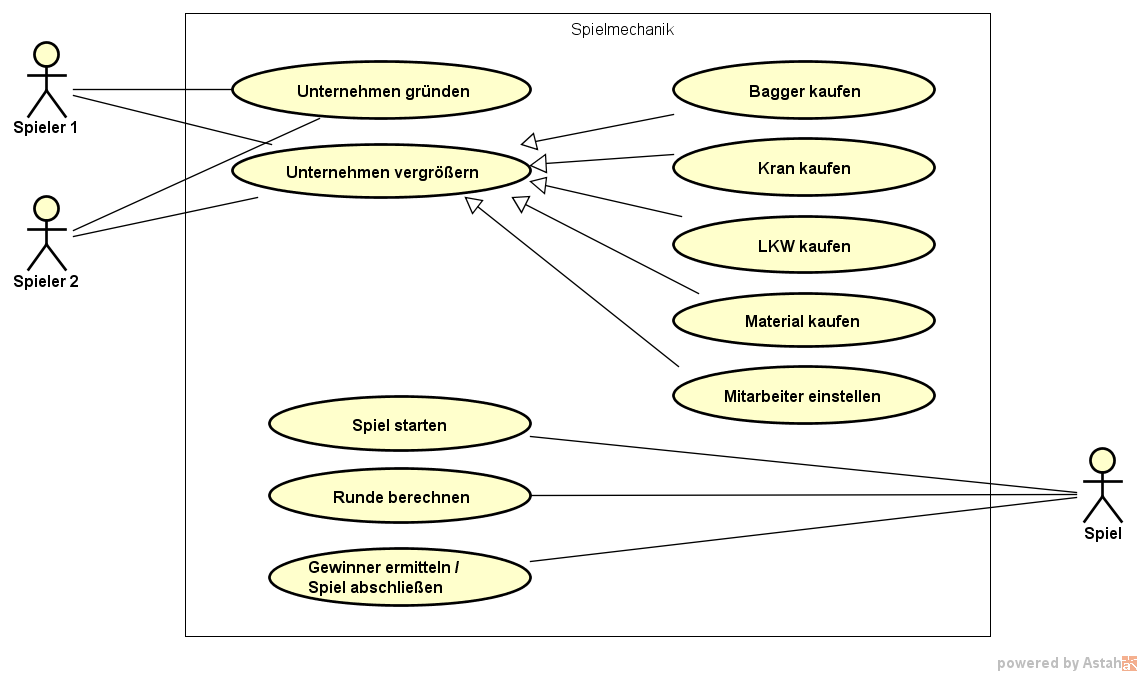
\includegraphics[scale=0.4]{img/UseCasePrototypeFallstudie.png}
	\captionof{figure}{\label{abb:usecase1}Use-Case Diagramm des ersten Prototypen}
	\vspace{2em}
\end{minipage}

\section{Klasssendiagramm}

Aus diesem Use-Case Diagramm ist dann folgendes Klassendiagramm entstanden:

\begin{minipage}{\linewidth}
	\centering
	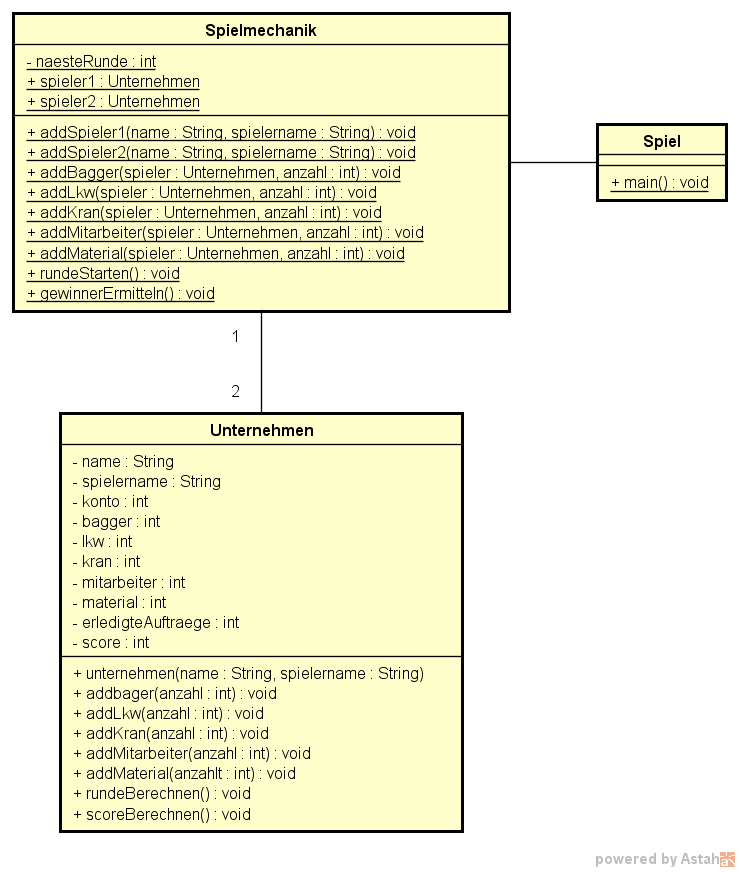
\includegraphics[scale=0.63]{img/ClassDiagramPrototypeFallstudie.png}
	\captionof{figure}{\label{abb:classdiag1}Klassendiagramm des ersten Prototypen}
	\vspace{2em}
\end{minipage}

Bei dieser Programmierung stellt die Klasse \glqq Unternehmen\grqq \ den Spieler samt seines Unternehmens dar. Die Klasse \glqq Spielmechanik\grqq \ erzeugt zum Spielstart die beiden Spieler, also zwei Instanzen der Klasse \glqq Unternehmen\grqq . Über die Klasse \glqq Spiel\grqq \ erfolgen die Eingaben an das Spiel. In ihr befindet sich auch die Main-Methode, die zum Spielstart ausgeführt werden muss. 

\section{Spiel Beispiel}

Ein mögliches Spiel wie es in der Klasse \glqq Spiel\grqq \ gespielt werden könnte, sieht zum Beispiel so aus:

\lstset{language=Java}
\begin{lstlisting}[caption={Beispiel für die Klasse \glqq Spiel\grqq}, label={lst:prototypspiel}]
public class spiel {

public static void main(String[] args) {

spielmechanik.addSpieler1("ABC Bau GmbH", "Daniel Pies");
spielmechanik.addSpieler2("XYZ Bau OHG", "Manuel Techert");

spielmechanik.addBagger(spielmechanik.spieler1, 2);
spielmechanik.addKran(spielmechanik.spieler1, 1);
spielmechanik.addLkw(spielmechanik.spieler1, 1);
spielmechanik.addMitarbeiter(spielmechanik.spieler1, 3);

spielmechanik.addBagger(spielmechanik.spieler2, 1);
spielmechanik.addKran(spielmechanik.spieler2, 1);
spielmechanik.addLkw(spielmechanik.spieler2, 2);
spielmechanik.addMaterial(spielmechanik.spieler2, 10);

spielmechanik.rundeStarten();

spielmechanik.addBagger(spielmechanik.spieler1, 2);
spielmechanik.addMitarbeiter(spielmechanik.spieler1, 5);

spielmechanik.addLkw(spielmechanik.spieler2, 2);
spielmechanik.addMaterial(spielmechanik.spieler2, 10);

spielmechanik.rundeStarten();

spielmechanik.gewinnerErmitteln();

}

}

\end{lstlisting}

%% !TEX root =  master.tex 
\chapter{Wirtschaftliche Aspekte im Spiel}  // ersetzt durch Nicos Kapitel

% !TEX root =  master.tex 
\chapter{Use-Case-Diagramm -- Gemeinsam}

Folgendes Use-Case-Diagramm ist im Laufe unseres Projektes entstanden:

\begin{minipage}{\linewidth}
	\centering
	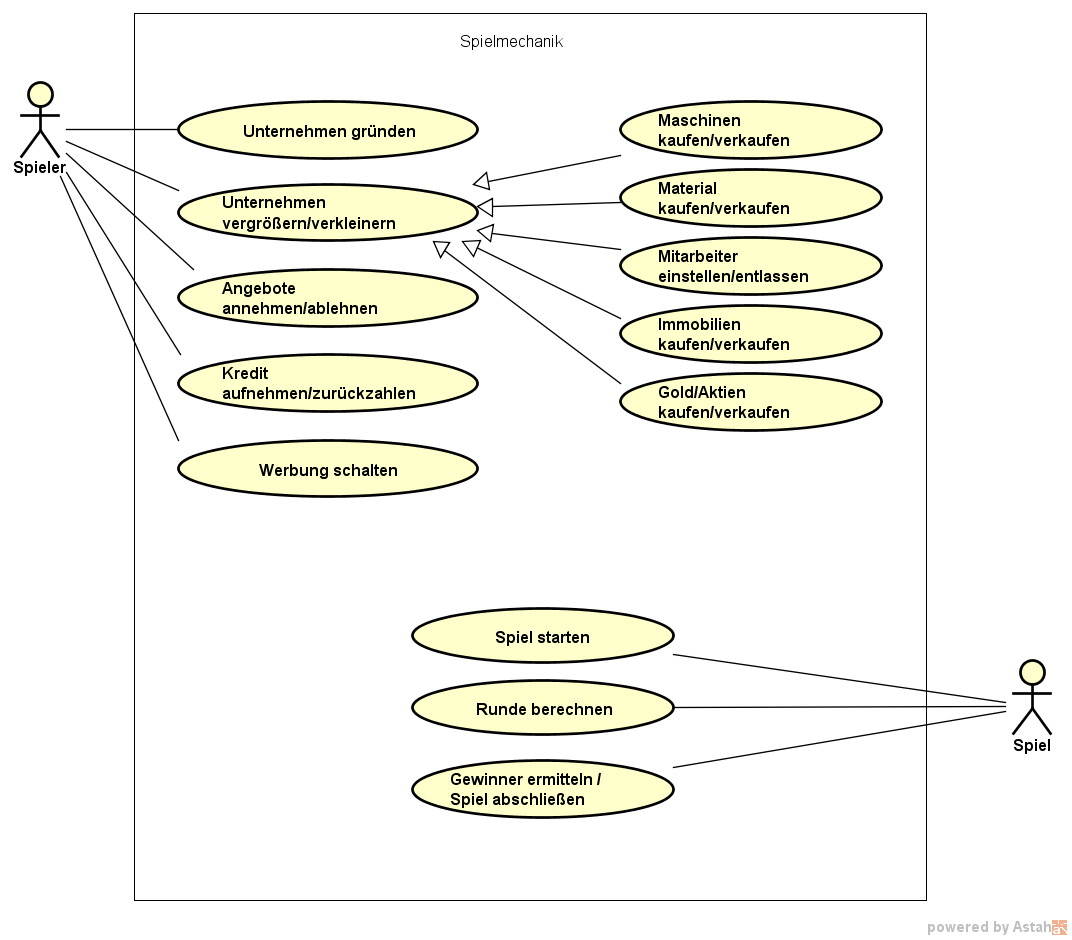
\includegraphics[scale=0.55]{img/UseCasezweiteIterationFallstudie.png}
	\captionof{figure}{\label{abb:usecase2}Finales Use-Case Diagramm}
	\vspace{2em}
\end{minipage}

% !TEX root =  master.tex 
\chapter{Fachkonzept und Programmierung -- Nico Popiolek}

\section{Die Klasse Unternehmen}
Kernstück des Fachkonzepts bildet die Klasse Unternehmen, welche alle relevanten Daten, Eigenschaften und Funktionen des Unternehmens beinhaltet. Dazu zählen sowohl Anlage- wie Umlaufvermögen, als auch virtuelle Werte der Spielmechanik wie eine Statistik oder der Einfluss des Marketings. Zwischen jedem Unternehmen und Spieler besteht eine 1 zu 1 Beziehung, es ist also nicht möglich für einen Spieler, mehrere Unternehmen in der gleichen Runde zu verwalten und ebenso gibt es keine Unternehmen, welche 'autonom' bzw. von der Spielmechanik gesteuert am Spiel teilnehmen.

Es wurden die folgenden Attribute eines Unternehmens in das Fachkonzept integriert:

\begin{itemize}
	 
\item Immobilien, leider konnte die Klasse jedoch aufgrund Zeitmangels nicht vollständig implementiert werden. Das Fachkonzept sah vor, dass ein Unternehmen ab einer bestimmten Anzahl Mitarbeiter und Lagerbestände weitere oder größere Immobilien erwerben muss, um den Betrieb aufrecht zu erhalten. So erhält der Spieler lediglich eine Immobilie mit einem Wert von 1.600.000\euro zu Beginn des Spiels, welche dann mit jeder Runde abgeschrieben wird bis auf einen Wert von einem Euro, sonst jedoch keine weitere Funktion erfüllt.

\item Baumaterialien, welche in Form von Stahl, Beton und Holz gehandelt und verwendet werden können. Dafür wurde eine ArrayList implementiert, welche die drei Rohstofftypen als Objekte beinhaltet. Bei Kauf oder Verwendung der Materialien wird jeweils die Variable \texttt{anzahl} verändert. Es stehen die Materialien Holz, Beton und Stahl zu Verfügung, welche alle in Tonnen gehandelt werden. Als grober Richtwert für ein mehrstöckiges Einfamilienhaus wurden 21t Holz, 10t Stahl und 100t Beton angenommen, deren Nettopreise in Deutschland aktuell bei etwa 100\euro, 500\euro und 30\euro  liegen.

\item Baumaschinen, welche als Bagger, Kräne und LKWs gehandelt und auf den Baustellen eingesetzt werden können. Anders als bei den Baumaterialien existiert hier eine ArrayList, welche jede einzelne Baumaschine als individuelles Objekt beinhaltet. Diese Vorgehensweise war nötig, da Maschinen funktional komplexer sind als Baumaterialien. So erhält jede Maschine ein Attribut \texttt{inVerwendung}, welches kennzeichnet, ob die Maschine gerade auf einer Baustelle im Einsatz ist, oder für neue Aufträge zur Verfügung steht. Des weiteren hat jede Baumaschine einen Wert, welcher zu Anfang dem Kaufpreis entspricht und dann jährlich um 1/8 abgeschrieben wird. Die günstigste Baumaschine ist der Lkw mit einem Neupreis von 80.000\euro, danach folgt der Bagger mit 150.000\euro und am teuersten ist der Kran mit 170.000\euro. Nach Ablauf der acht Jahre, verbleiben die Maschinen weiter mit dem Wert von einem Euro als Anlagevermögen in der Bilanz.

\item Wertpapierdepots, welche dem Spieler die Möglichkeit geben, in Aktien oder Gold zu investieren. Die Entwicklung des Aktienmarkts orientiert sich dabei an jener der Gesamtwirtschaft und führt zu Kursveränderungen und Dividendenausschüttungen an den Spieler. So erhält das Unternehmen bei einem Wert unter 50 keinerlei Dividende seiner Aktien und muss Kursverluste hinnehmen, bei einer guten Wirtschaftslage über 50 steigt der Wert der Aktien und eine jährliche Dividende, die vom aktuellen Marktscore abhängt, wird ausgezahlt. Umgekehrt verhält es sich mit Investitionen in Gold. Es wird angenommen, dass Anleger bei schlechter Wirtschaftslage und fallenden Aktienkursen verstärkt in Gold investieren, was zu einer Kurssteigerung führt und umgekehrt. So kann der Spieler sich absichern, falls er einen größeren Wirtschaftscrash befürchtet. Bei einer langsam und kontinuierlich wachsenden Wirtschaft profitieren sowohl der Aktienmarkt als auch der Kurs von Gold. Eine Dividende auf Gold wird nicht ausgezahlt.

\item Kredite werden grundsätzlich in Form von Tilgungsdarlehen an die Spieler ausgegeben. Die jährlichen Rückzahlungen beinhalten sowohl den gleichbleibenden Tilgungsanteil, welcher sich aus der Kreditsumme und der Laufzeit ergibt als auch den Zinsanteil, welcher jährlich neu berechnet und auf 5\% der verbleibenden Kreditsumme gesetzt wird. Die Summe und Laufzeit kann der Spieler selbst auswählen, eine vorzeitige Tilgung des Kredits ist jedoch nicht vorgesehen.

\item Bauarbeiter, wobei hier unterschieden wird zwischen solchen, die aktuell auf einer Baustelle aktiv sind und freien Bauarbeitern, welche für eingehende Angebote zur Verfügung stehen. Inklusive Lohnnebenkosten fallen pro Bauarbeiter Kosten in Höhe von 50.000 Euro pro Jahr an. Für das Entlassen eines Bauarbeiters müssen unabhängig von seinem Status 15.000\euro Abfindung gezahlt werden. Hat ein Bauarbeiter auf einer Baustelle einen tragischen Arbeitsunfall, kann er zusätzlich Schmerzensgeld verlangen, im Falle einer permanenten Invalidität oder sogar Tod des Angestellten, werden hohe Schmerzensgeldzahlungen fällig und die Anzahl der Bauarbeiter wird um eins verringert.

\item Verwaltungsangestellte sind bei wachsender Größe des Unternehmens zunehmend notwendig und verursachen Kosten von 55.000 Euro pro Mitarbeiter und Jahr. Soll ein Verwaltungsangestellter entlassen werden, so muss das Unternehmen ihm 18.000\euro Abfindung zahlen. Bis zum Zeitpunkt der Fertigstellung dieses Projekts konnten leider keine weitere den Spielablauf beeinflussenden Funktionen für Verwaltungsangestellte implementiert werden. Ursprünglich war angedacht, dass das Unternehmen bei wachsender Größe auch mehr Verwaltungsangestellte benötigt und diese gegebenenfalls auch weitere spielerische Vorteile mit sich bringen, wie beispielsweise erfolgreichere Marketingkampagnen.

\item Bankkonto, welches die flüssigen Geldmittel des Unternehmens repräsentiert und somit den zentralen Knotenpunkt aller Geldflüsse darstellt. Alle Zu- und Abflüsse von Geld werden über das Bankkonto dargestellt, Kredite werden also beispielsweise direkt von der Bank auf das Konto des Unternehmens ausgezahlt und erst im zweiten Schritt für Investitionen verwendet. Gibt der Spieler mehr Geld aus, als auf dem Konto vorhanden ist, so rutscht dies zunächst im UI ins Minus. Wird die nächste Runde gestartet, so findet eine Prüfung auf den Kontostand statt und sollte dieser negativ sein, so wird automatisch ein Kredit über den Fehlbetrag aufgenommen, sodass der Spieler kein zinsloses Darlehen durch einfaches Geldausgeben erhält.

\item Marketing, welches dem Spieler unterschiedliche Formen des Marketings zu Verfügung stellt, die sich in Kapitalintensivität und Effektivität unterschieden und dem Spieler in Form eines Marketing-Scores einen Vorteil gegenüber anderen Spielern verschaffen können. Außerdem kann der Spieler seinen eigenen Marketingscore abfragen, wobei der relative Marketingscore Auswirkungen auf die eingehenden Aufträge des Spielers hat. Bei jeder Investition eines Spielers erhöht sich sowohl der eigene als auch der globale Marketingscore, welcher die Summer der Marketingscores aller Spieler ist, um den gleichen Wert. Damit steigt der eigene relative Anteil, wogegen der aller anderen Spieler gleichzeitig sinkt. Dieser Mechanismus soll einerseits die Konkurrenz unter den Spielern darstellen und ein Gegenseitiges Verdrängen ermöglichen und andererseits sicherstellen, dass die Nachfrage im Markt nicht von der Werbung der Unternehmen, sondern vielmehr von der wirtschaftlichen Lage, also dem verfügbaren Kapital der Kunden abhängt - ein erfolgreiches Marketing sichert dem Spieler lediglich ein größeres Stück des nach wie vor gleich großen Kuchens zu. Ein hoher relativer Marktanteil bedeutet dennoch signifikante Vorteile gegenüber den anderen Mitspielern.

\end{itemize}

Es wird davon ausgegangen, dass jeder Spieler zu Beginn des Spiels mit einem sehr kleinen oder neuen Unternehmen, aber großer Kapitaldecke startet. Deshalb wird jedes neue Unternehmen im Konstruktor mit einer Immobilie, einem kleinen Aktiendepot, ein paar Angestellten, Rohstoffen für eine kleine bis mittlere Baustelle und je einer Baumaschine jedes Typs sowie 5 Millionen Euro auf dem Konto initialisiert. So sieht der Spieler gleich zur ersten Runde was mit welchen Positionen im UI passiert und kann durch die große Menge liquider Mittel das Unternehmen nach seinen Präferenzen aufbauen und bereits früh entscheiden, ob er beispielsweise auf einer Verdrängungsstrategie der anderen durch große Investitionen in Marketing setzt, auf Wertpapiere als zweites Standbein oder schnelles Wachstum durch Kauf von Material und Maschinen und Annahme möglichst großer Aufträge.


\section{Steuerung und Spielablauf}
Die teilnehmenden Unternehmen werden verwaltet über die Klasse Unternehmensverwaltung. Die Unternehmensverwaltung ist ein Singleton und enthält eine ArrayList mit allen Unternehmen und stellt Methoden bereit, mit denen die Funktionen der Unternehmen ausgeführt werden können. Analog dazu wurden auch die Angebotsverwaltung sowie der GameEventHandler und GameEventGenerator als Singletons implementiert.
Die Angebotsverwaltung dient dazu, neue Angebote zu generieren, anzunehmen, abzulehnen und ihre Dauer zu verwalten. Zusätzlich werden hier Events erzeugt, die sich auf bereits angenommene Angebote auswirken, wie zum Beispiel eine Verlängerung der Baustelle durch bestimmte Ereignisse.
Jeder Spieler erhält pro Runde drei Angebote. Diese unterliegen sowohl in ihrer Größe als auch ihrer Rentabilität Zufallswahrscheinlichkeiten, die sich in vorgegebenen Korridoren bewegen und durch die aktuelle Konjunktur sowie den relativen Marketingscore des Unternehmens beeinflusst werden. Zunächst wird für jedes Angebot eine von drei möglichen Größen 1 bis 3 zufällig ermittelt. Ein Angebot der Kategorie 1 entspricht dem kleinstmöglichen Angebot und orientiert sich an  dem Umfang eines normalen Einfamilienhauses. Kategorie 2 entspricht einer ungefähr doppelt so großen Baustelle und Kategorie verlangt noch einmal etwa den dreifachen Materialeinsatz.
Entsprechend der Größe wird nun für alle benötigten Ressourcen und auch den Preis in definierten Grenzen Zufallswerte ermittelt und schließlich um den Konjunktur- und Marketingmodifikator verändert. Hat ein Unternehmen einen besonders hohen relativen Marketingscore, sind die Angebote wesentlich lukrativer als die der Konkurrenz. Das fördert einerseits den Anreiz, mehr Geld in Marketing zu investieren, um so die anderen Spieler auszustechen und bessere Angebote zu erhalten und andererseits zwingt es die Spieler dazu, jedes Angebot einzeln genau zu prüfen, denn unabhängig von der Größe und Marktsituation kann ein Angebot für den gegebenen Preis einen höheren oder niedrigeren Material- und Arbeitseinsatz verlangen und somit mehr oder weniger lukrativ sein. Insbesondere die Lohnkosten sind hier als entscheidender Faktor zu berücksichtigen, zusätzlich aber auch Kosten für unvorhergesehene Ereignisse wie ein Wasserrohrbruch mit einzukalkulieren. Alle Grenzen wurden jedoch so gesetzt, dass kein Angebot von vornherein einen sicheren Verlust erzielt, da ein reales Unternehmen einen solchen Auftrag nicht annehmen würde. Angebote können grundsätzlich nur angenommen werden, wenn alle benötigten Rohstoffe, Baumaschinen und Bauarbeiter zu Beginn an vorhanden sind. Zuführen weiterer Ressourcen während der Bauzeit ist nicht möglich und da eine Runde etwa einem verstrichenen Jahr entspricht, sind alle Angebote nur genau eine Runde lang gültig. Entscheidet sich der Spieler ein Angebot nicht anzunehmen, wird es nicht wieder auftauchen und stattdessen durch neue Angebote ersetzt.

Durch ein oder mehrere unvorhergesehene Events kann eine Baustelle jedoch zum Verlustgeschäft werden - auch hier muss der Spieler planen und abwägen, ob zum gegebenen Preis ausreichend Puffer vorhanden ist.
Nimmt der Spieler ein Angebot an, werden ihm am Ende der Runde alle benötigten Rohstoffe abgezogen und die Anzahl benötigter Bauarbeiter und Maschinen stehen für die Dauer der Baustelle nicht zur Verfügung. Während der Bauphase werden zusätzlich in jeder Runde Wahrscheinlichkeiten für diverse Zufallsevents auf den Baustellen generiert. Dies reicht von einem Wasserschaden, welcher lediglich einen geringen finanziellen Verlust für den Spieler bedeutet bis hin zu Events wie dem Auffinden geschützter Tierarten auf dem Baugrundstück, was eine Verlängerung der Bauzeit um ein Jahr bedeutet und für den Spieler hohe Lohnkosten und den Verzicht auf Bauarbeiter und Maschinen nach sich zieht. Ebenfalls möglich sind Arbeitsunfälle, welche zu Schmerzensgeldzahlungen und im schlimmsten Fall sogar zum permanenten Verlust eines Bauarbeiters führen können. Sämtliche Events werden dem Spieler im UI in Textform dargestellt.
Erreicht die verbleibende Bauzeit null, werden die Bauarbeiter und Maschinen wieder verfügbar für neue Aufträge und der gesamte Preis des Angebots wird dem Konto gutgeschrieben. Es findet keine An- oder Ratenzahlung statt.

Der GameEventGenerator stellt die Methode \texttt{generiereWahrscheinlichkeit} zur Verfügung, welche an vielen anderen Stellen verwendet wird, der Handler ist dafür zuständig, die globalen Events zu verwalten und beispielsweise das Wirtschaftsklima jede Runde zu errechnen. Aufgrund Zeitmangels konnten hier neben der jährlichen Veränderung des Wirtschaftsklimas keine weiteren Events implementiert werden. Ideen waren beispielsweise ein branchenweiter Streik der Bauarbeiter welcher alle Spieler betrifft und längere Bauzeiten sowie höhere Löhne zur Folge hat, ein Börsencrash, Zinsveränderungen und schwankende Rohstoffpreise.

Die Klasse \texttt{Spiel}, welche den Spielablauf nach jeder Runde steuert, greift in der zentralen Methode \texttt{starteRunde} auf die Singletons zu und führt so in logischer Reihenfolge die nötigen Operationen zwischen den einzelnen Runden aus. Dazu zählen die Abrechnung der Gehälter, Abschreibungen, Aufnahme und Rückzahlung der Kredite, die Berechnung der neuen Aktienkurse mit der zugehörigen Dividendenausschüttung und zum Schluss die Berechnung des neuen Eigenkapitals für alle teilnehmenden Unternehmen, welches in der Bilanz verwendet wird. Während der Programmierung war es außerdem Konvention, alle Exceptions einheitlich in der \texttt{Spiel}-Klasse zu behandeln um die Übersicht und Wartbarkeit des Projekts zu verbessern.

Die Eingabewerte unterteilen sich in solche, die direkt nach ihrer Eingabe verwaltet werden - dazu zählt die Manipulation der Mitarbeiter, Maschinen, Baumaterial und Kredite - und solche, die erst nach Ende der Runde verarbeitet werden. Diese Entscheidung wurde getroffen, damit der Spieler während einer Runde auf die ihm gegebenen Angebote reagieren kann und gegebenenfalls Material oder Maschinen einkaufen kann, um einen besonders lukrativen Auftrag annehmen zu können, welcher andernfalls nach Ende der Runde nicht mehr zur Verfügung stünde, da alle Angebote neu generiert wurden.

Nachdem alle Berechnungen abgeschlossen wurden, wird nun an dieser Stelle der Rundenzähler erhöht und zum Spielende der Gewinner ermittelt.



 % // ACHTUNG muss noch fertig geschrieben werden

% !TEX root =  master.tex 
\chapter{UML-Diagramm -- Gemeinsam}

Da unser UML-Diagramm sehr groß ist, befindet sich hier ein Diagramm, das nur die vorhanden Klassen und deren Beziehungen beinhaltet:

\begin{minipage}{\linewidth}
	\centering
	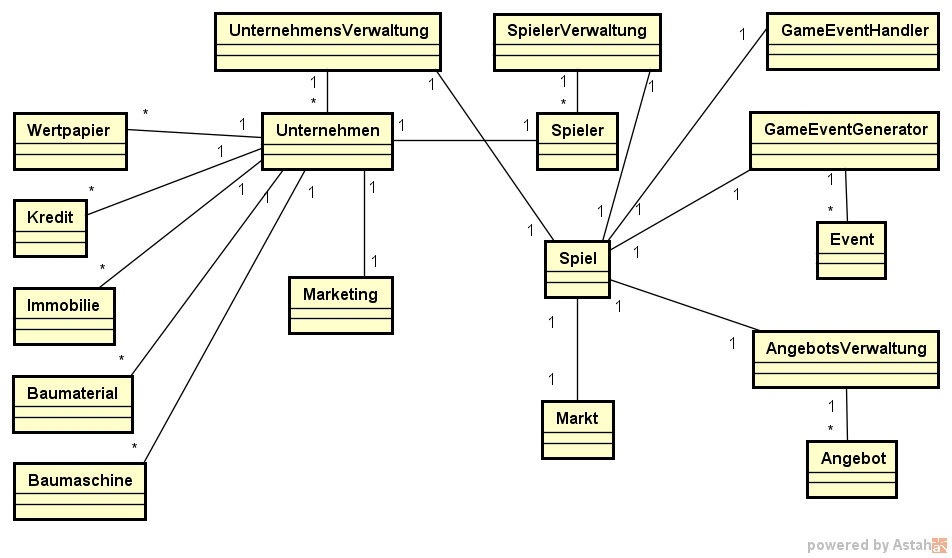
\includegraphics[scale=0.63]{img/ClassDiagramzweiteIterationFallstudieUEbersicht.png}
	\captionof{figure}{\label{abb:class1}UML-Diagramm (Klassenübersicht)}
	\vspace{2em}
\end{minipage}

Das vollständige UML-Diagramm befindet sich auf der nächsten Seite. Das Diagramm liegt zur besseren Lesbarkeit auch in digitaler Version vor.

\begin{minipage}{\linewidth}
	\centering
	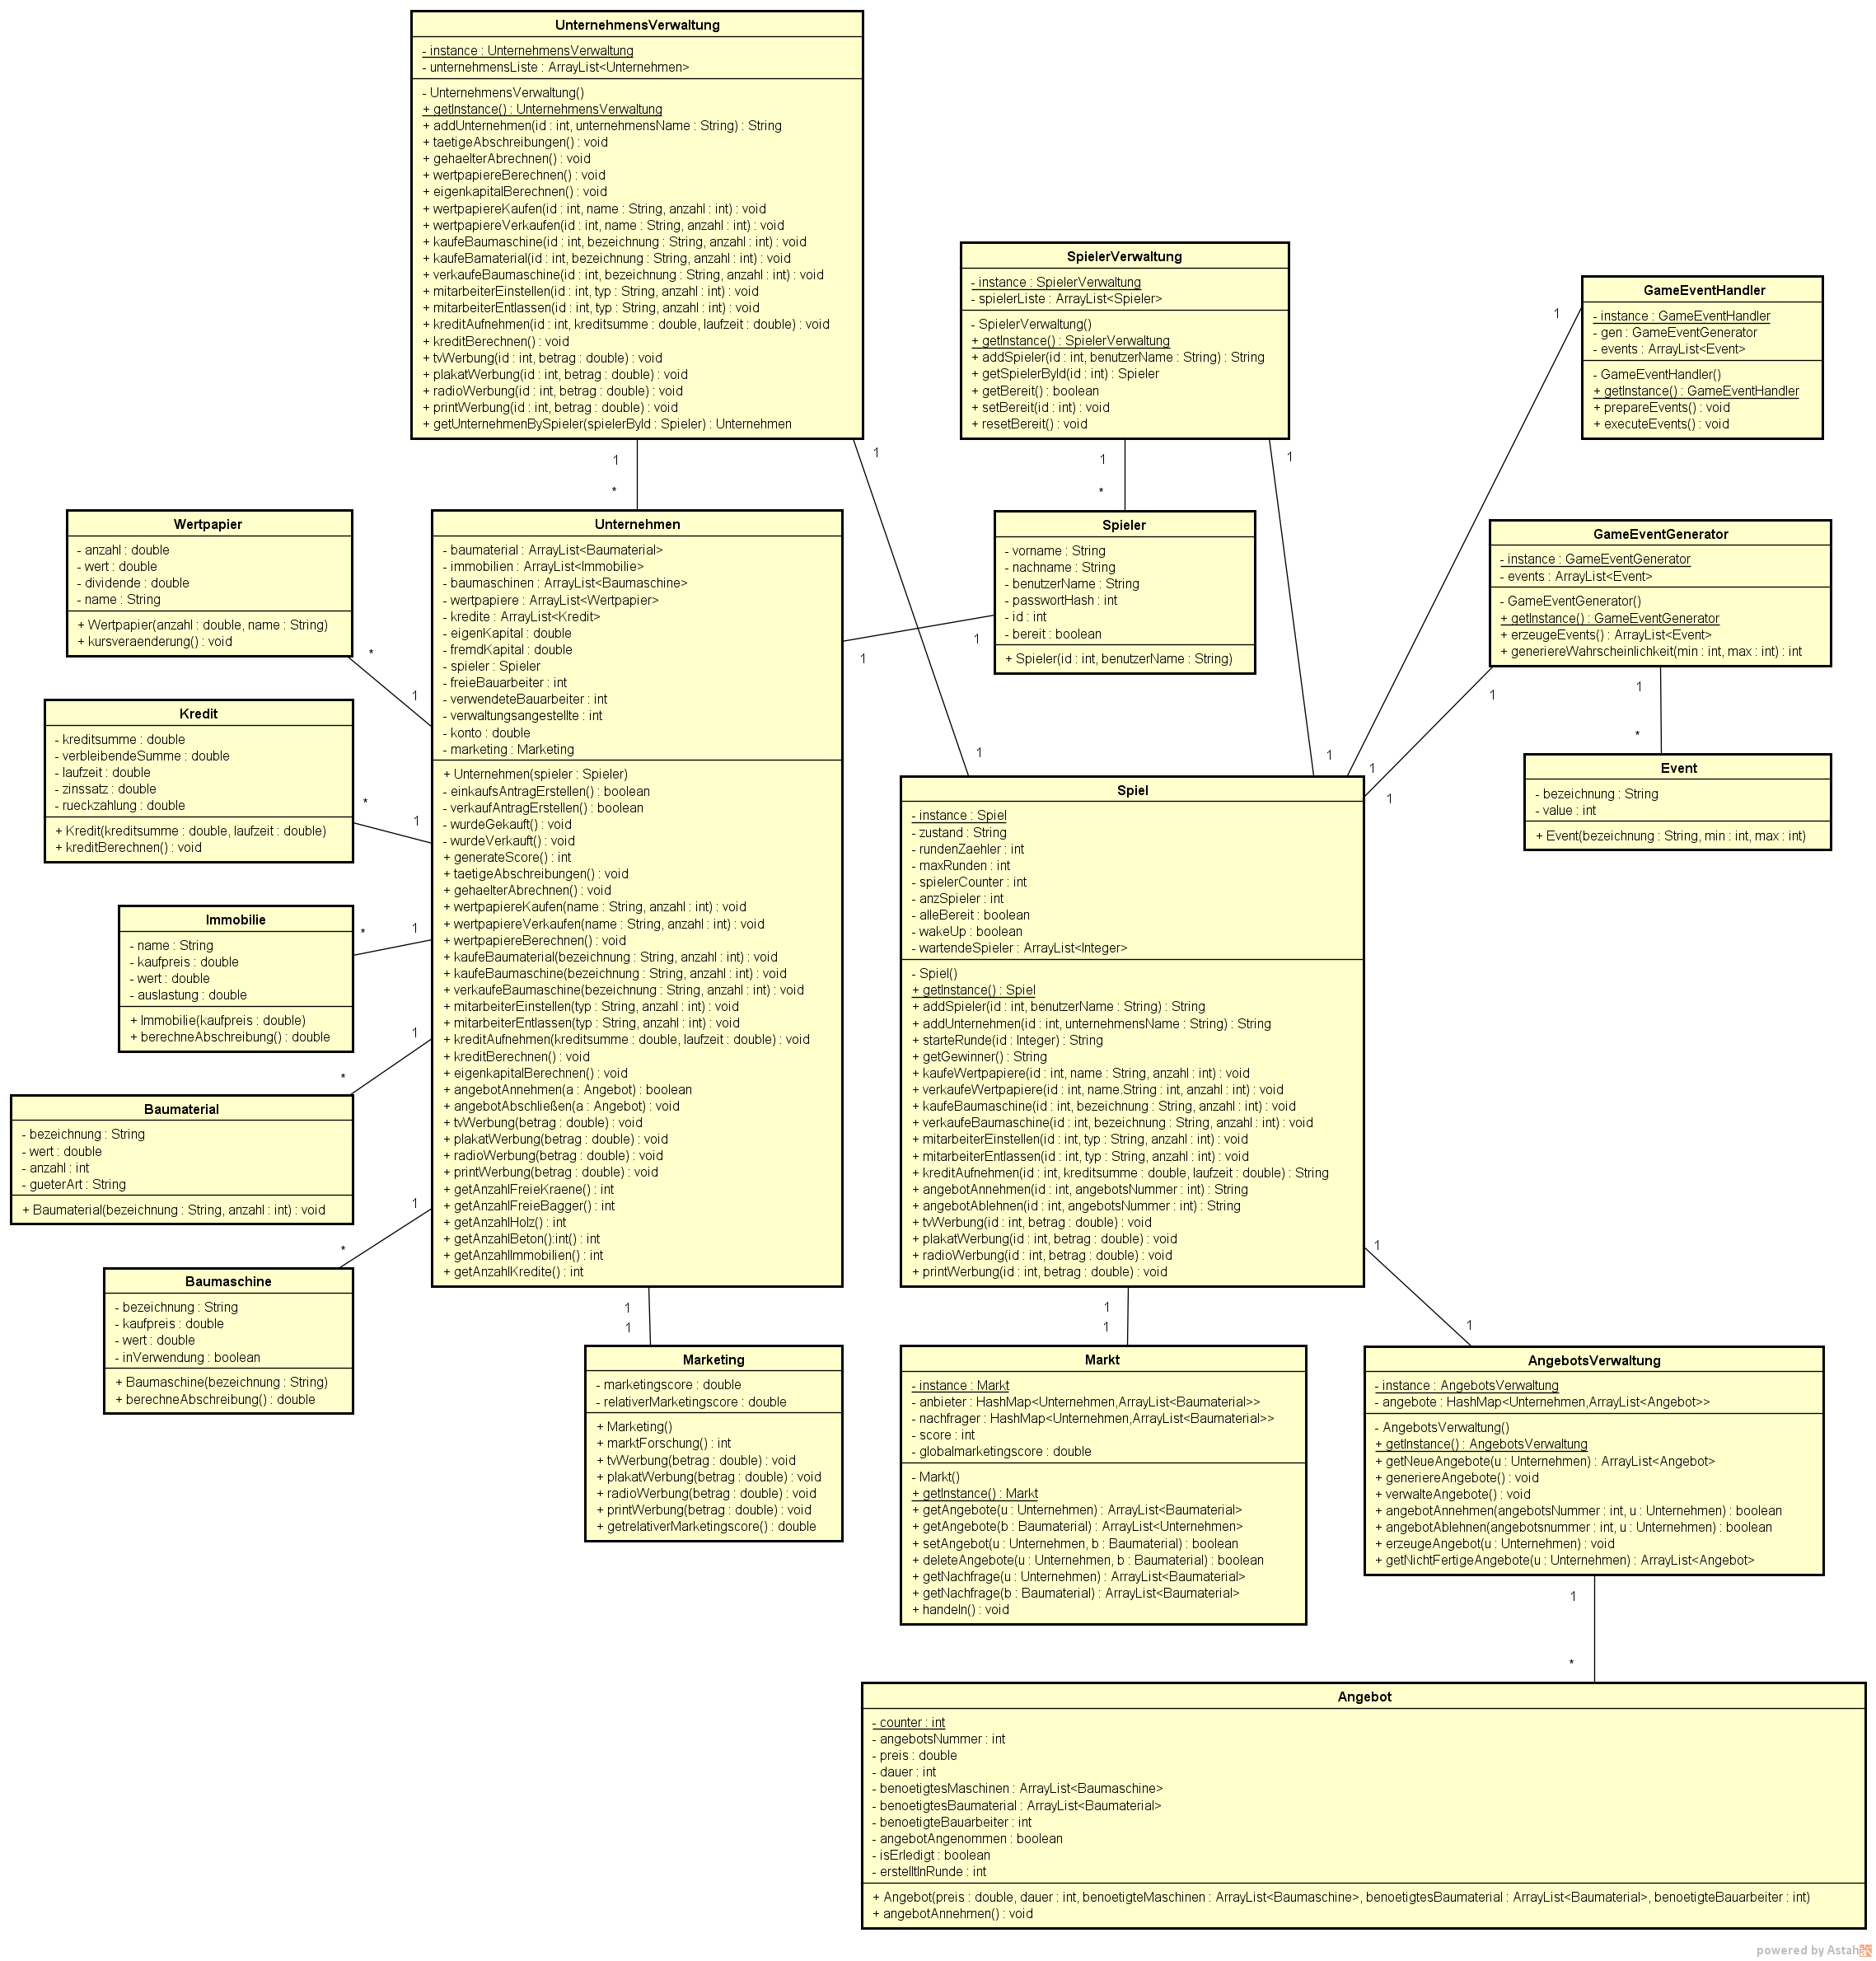
\includegraphics[scale=0.25]{img/ClassDiagramzweiteIterationFallstudie.png}
	\captionof{figure}{\label{abb:class2}UML-Diagramm}
	\vspace{2em}
\end{minipage}  % // ACHTUNG muss unbedingt noch eingefügt werden

% !TEX root =  master.tex 
\chapter{Erstellen des Mockups -- Manuel Techert}

\section{Erstellen des ersten Mockups}

Um eine Vorstellung davon zu bekommen, wie unsere Benutzeroberfläche später einmal aussehen soll, wollten wir vorhandene Ideen visualisieren. Dazu benutze ich Sketch, ein Design-Tool für macOS, welches das Gestalten von Oberflächen aller Art ermöglicht.

Zunächst sollen zwei verschiedene Situationen visualisiert werden - Das Log-in Fenster und das Spielefenster.

Bei dem Log-In Fenster sollen zwei Eingabefenster realisiert werden. Da das Spiel nicht lokal, sondern über mehrere Computer gespielt werden kann, habe ich eine einfache Anmeldemaske mit zwei rechteckigen Feldern mit den Eingaben Benutzername und Passwort erstellt.
Nach erfolgreichem Anmelden auf dieser Maske, soll der Benutzer zum eigentlichen Spiel weitergeleitet werden. Diese Oberfläche stellt das Spielefenster dar.

Hier muss es dem Spieler möglich sein, wichtige Informationen abzurufen und alle nötigen Interaktionen durchzuführen. Realisiert ist dies in einem an ein normales Chat-Fenster angelehntes Protokoll, in welchem wichtige Vorgänge mit einem Zeitstempel notiert werden.

In der Sparte rechts daneben finden sich die wichtigsten Informationen zum aktuellen Geschene wieder - darunter zum Beispiel der Kontostand und die Aufträge, die der Spieler momentan als Unternehmen hat.

Darunter befinden sich mehrere Buttons, die die Interaktion des Spielers mit dem Spiel ermöglichen. Zur besseren Verwertung werden als Platzhalter die Buttons Bagger, LKW und Mitarbeiter implementiert, dessen Anzahl sich mit dem sich daneben befindenden Knopf erhöhen lässt.

Nachdem das Mockup fertiggestellt ist, wird es als PNG-Datei exportiert, um es in der ersten Iteration vorstellen zu können.
Im nächsten Schritt soll das Mockup in HTML und CSS umgesetzt und so stetig ausgebaut werden.


\begin{minipage}{\linewidth}
	\centering 
	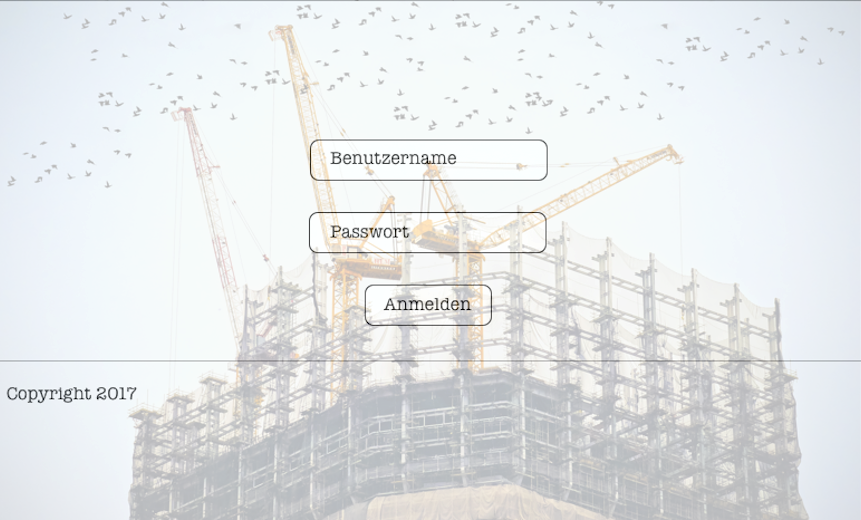
\includegraphics[scale=1]{img/Mockup1Teil1.png}
	\captionof{figure}{\label{abb:mockup1.1}Das erste Mockup}
	\vspace{2em}
\end{minipage}


\begin{minipage}{\linewidth}
	\centering 
	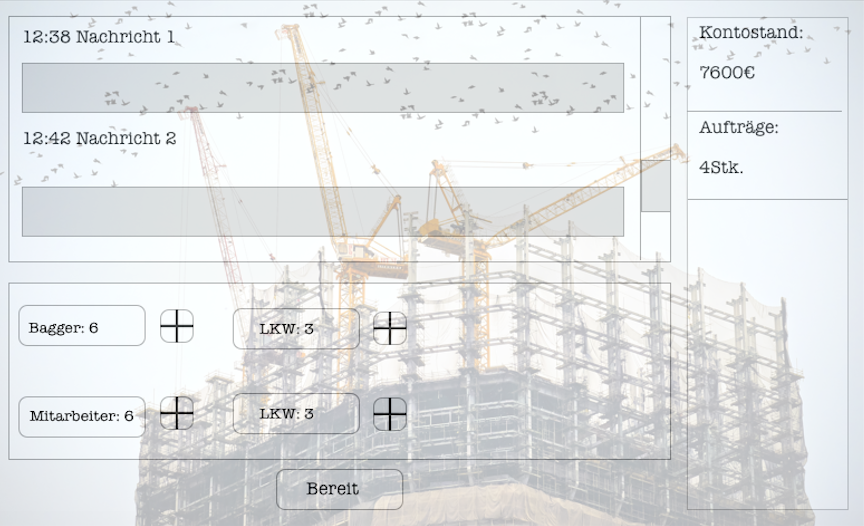
\includegraphics[scale=1]{img/Mockup1Teil2.png}
	\captionof{figure}{\label{abb:mockup1.2}Das erste Mockup}
	\vspace{2em}
\end{minipage}


% !TEX root =  master.tex 
\chapter{Mockup des UIs mit html -- Daniel Pies}

\section{Übersicht}

Unser zweites Mockup des Spiels haben wir mit html erstellt, um es mithilfe eines Webservers aufrufen zu können, da auch unser Spiel mittels eines Webservers auf verschiedenen Geräten gestartet werden kann. Das Mockup sollte alle Informationen erhalten, die der Spieler auch im fertigen Spiel als Entscheidungshilfe haben soll. Dazu bietet es sich an ein Grid-Layout zu verwenden, das mehrere Elemente auch nebeneinander anzeigen kann. Die html-Seite besteht hauptsächlich auch drei Spalten, wobei der Bereich der Spielereingaben noch einmal in drei Spalten unterteilt ist.


\begin{minipage}{\linewidth}
	\centering
	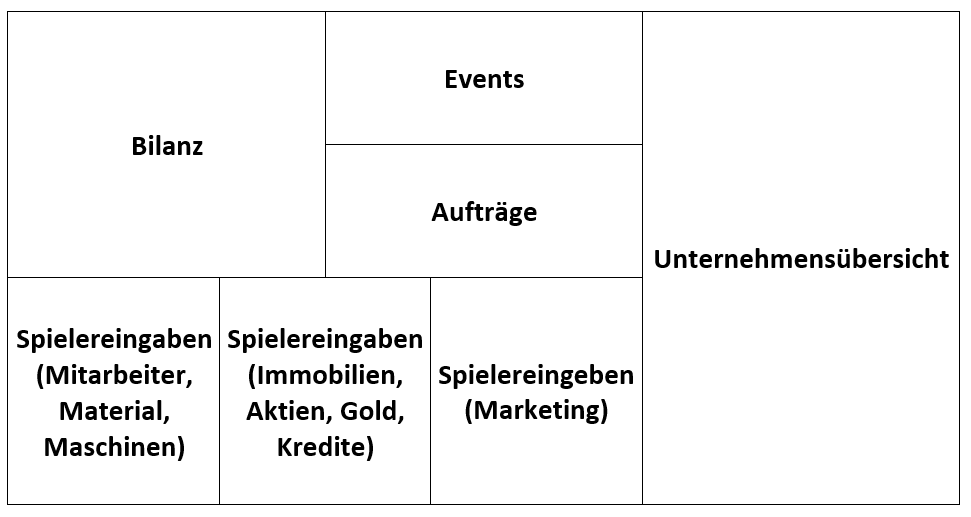
\includegraphics[scale=0.6]{img/Uebersicht.png}
	\captionof{figure}{\label{abb:aufbauhtml}Aufbau des html-Mockups}
	\vspace{1em}
\end{minipage}

\newpage

\section{Die wichtige Elemente}

Die wichtigen Elemente im UI sind:

\begin{description}
	\item[Die Übersicht]\hfill \\
	Hier sieht der Spieler die kompletten Informationen zu seinem Unternehmen. Alle Werte wie Kontostand, Immobilien, Bauarbeiter, Verwaltungsangestellte, Baumaschinen, Baumaterialen, Aktien, Gold, Kredite, Marketingscore und alle aktiven Baustellen sind detailliert aufgelistet.
	\item[Die Bilanz]\hfill \\
	Hier findet der Spieler die Bilanz seines Unternehmens analog zur Finanzbuchhaltung. Der Spieler hat einen finanziellen Überblick und sieht, ob er beispielsweise Investieren kann oder knapp bei Kasse ist.
	\item[Die Events]\hfill \\
	Hier stehen informative Texte zur letzter Runde, die den Spieler bei der nächsten Runde unterstützen können. Solche Texte sind zum Beispiel \glqq Das letzte Jahr war sehr erfolgreich. Die Wirtschaft erlebt einen deutlichen Aufschwung. Die Auftragslage ist weiterhin sehr gut.\grqq \ oder \glqq Im Stadtteil Eastside gab es einen Wasserrohrbruch. Zwei deiner Baustellen verzögern sich um einige Zeit.\grqq
	\item[Die Aufträge]\hfill \\
	Hier findet der Spieler alle für ihn zur Verfügung stehenden Aufträge inklusive der Benötigten Materialien, Maschinen und Mitarbeiter um den Auftrag auszuführen. Durch einen Button kann der Spieler den Auftrag annehmen.
	\item[Die Spielereingaben]\hfill \\
	Hier hat der Spieler die Möglichkeit so ziemlich alle Werte seines Unternehmens anzupassen. Er kann hier Mitarbeiter einstellen oder entlassen; er kann Maschinen anschaffen oder Baumaterial kaufen; er kann Kredite aufnehmen oder Gold kaufen; oder kann in das Marketing seines Unternehmens investieren, um nur einige Möglichkeiten zu nennen. Diese Interaktionen des Spielers funktionieren mit \glqq +\grqq- oder \glqq -\grqq-Buttons oder durch die direkte Eingabe der gewünschten Zahl.
\end{description}


% !TEX root =  master.tex 
\chapter{Server-Client Architektur -- Fabian Pulch}

\section{Grundlegende Überlegungen}
Der Aufbau des Planspiels soll zuvor bereits beschrieben multiplayerfähig sein und von mehreren Spielern, jeder jeweils ausgestattet mit einem eigenen Client, spielbar sein. Da man sich gegen ein \glqq Hot Seat\grqq \  Verfahren entschieden hat, wurden Überlegungen hinsichtlich einer Server-Client Architektur getroffen, welche im folgenden erläutert werden. Kernproblemstellung dieses Kapitel ist die Frage, wie die Kommunikation zwischen Server und Client aussehen soll.

\section{Erster Ansatzpunkt}
Zunächst einmal wurde überprüft, ob die Programmiersprache Java, welche zur Implementierung des Projektes ausgewählt wurde, über eigene bereits integrierte Bibliotheken zur Kommunikation via TCP/IP verfügt. Im OSI Referenzmodell ist die Kommunikationslogik des Planspiels in der Anwendungsschicht anzusiedeln und den Transport, Internet und Netzzugriffsschichten dadurch übergeordnet.
%Abbildung zum TCP/IP Modell / OSI Modell einfügen
Java bietet in dem Paket \glqq java.net\grqq \ eine grundlegende Bibliothek an, um über mithilfe sogenannter Sockets über Protokolle wie TCP/IP kommunizieren zu können. Eine Nutzung dieser bereitgestellten Klassen und Interfaces hat den grundlegenden Vorteile, dass auf die Einbettung anderer Drittanbieter Codebibliotheken zur Kommunikationszwecken zwischen Server und Client meist gänzlich verzichtet werden kann. Dadurch bleiben die Systemvoraussetzungen minimal auf eine funktionsfähige Javalaufzeitumgebung beschränkt.  Ein Abhängigkeitsmanagement ist dadurch nicht unbedingt erforderlich.

Java als funktionsfähige Laufzeitumgebung auf Server als auch auf dem Client ist eine Möglichkeit mit Java Bordmitteln das Spiel zu realisieren. Dabei müsste der User allerdings in diesem Fall den Client zur Verfügung gestellt bekommen. Eine zuverlässige Verteilungsmethode des Client müsste also gewährleistet werden. Dies kann beispielsweise mithilfe eines Downloads oder der Übergabe auf einem USB-Stick oder einer CD geschehen. Diese Bereitstellung des Clients ist jedoch nicht sonderlich zeitsparend und benutzerfreundlich, da gegebenenfalls Java, falls noch nicht auf dem für den Client ausgewählten Endgerät installiert, nachgeladen werden muss. Durch diese Problematik mit dem Server und Client als eigenständige Java-Anwendung, wurde die Betrachtung weiterer Alternativen angestrebt.

\section{Zweiter Ansatzpunkt}
Da der erste Ansatz, die Problematik nicht vollständig zufriedenstellend löst, wurde nach einer weiteren Möglichkeit zur Realisierung der Kommunikation gesucht, welche einerseits eine zuverlässige Kommunikation zwischen Client und Server ermöglicht und andererseits für den Endbenutzer einfach zu bedienen ist. Im Laufe der Konzeption ist man auf das Konzept der Websockets in HTML5 gestoßen. Websockets benutzen das sog. Websocketprotokoll \autocite[vgl.][]{WebSocketProtokoll}. Mithilfe dieses Protokoll kann bidirektional zwischen einem Client (in diesem Fall eine Webanwendung) und einem Server (beispielsweise einem Webserver). Das Websocketprotokoll ist in der Anwendungsschicht im TCP/IP Protokollstack anzusiedeln. Die Spielschnittstellenkommunikation, welche regelt welche Daten der Client empfangen soll, in welchem Format etc. und welche Anfragen der Client an den Server schicken kann (beispielsweise \glqq starteRunde\grqq) setzt die Kommunikation in diesem Fall über das Websocketprotokoll voraus. Der vorher beschriebene erste Ansatz setzt lediglich eine etablierte TCP-Verbindung voraus.
Der wesentliche Vorteil der Nutzung von Websockets zur Kommunikation ist die Möglichkeit eine Webanwendung zu bauen. Im Gegensatz zu dem vorherigen Versuch ist dadurch kein Client, welcher in Java geschrieben wird, notwendig. Bei dieser Implementierungsmöglichkeit wird ein Client in Javascript ermöglicht. Dieser Client bietet den grundlegenden Vorteil, welcher mit dem Einsatz einer Webanwendung einhergeht, dass er beim jedem Aufruf der Webanwendung im Hintergrund auf das Endgerät geladen wird. Die Verteilung der benötigten Clientressourcen ist demnach unkomplizierter, als die Ausgabe eines reinen nativen Javaclienten.

Aufgrund dieser Überlegungen wurde der Entschluss getroffen eine Webanwendung zu entwerfen, anstatt eine native Java Server-Client Anwendung zu entwickeln.

Mit dieser Entscheidung wurde allerdings die Frage aufgeworfen, welche Implementierungsmöglichkeiten vorhanden sind. Nach einiger Recherche wurde eine erste Möglichkeit gefunden. Im folgenden werden die Überlegungen im Zusammenhang mit der Einordnung und Bewertung dieses Lösungsversuch erläutert.
\subsection{Server-Client Kommunikation mit dem Framework Spring und Websockets}
Um das Projekt zu verwalten und standardisieren, wird das Build-Management-Tool Maven\autocite[vgl.][]{Maven2} von der Apache Software Foundation genutzt. Dieses ermöglicht ein einfaches Management von Abhängigkeiten zwischen dem Projekt und diversen Softwarebibliotheken. Spring \autocite[vgl.][]{Spring}, eine Sammlung von Bibliotheken, welche die Entwicklung einer Webanwendung wesentlich erleichtern, wird durch Maven hinzugefügt. Durch die Einbindung von Spring ist ein Zugriff auf Bibliotheken möglich, die eine Kommunikation über das sogenannte STOMP Protokoll erlauben.\autocite[vgl.][]{SpringWithSTOMPExample} Dieses Protokoll basiert auf TCP und besitzt Ähnlichkeiten zu HTTP. Einige Befehle sind beispielsweise CONNECT, SEND, SUBSCRIBE, ACK oder DISCONNECT.
Diese Architektur ist vorteilhaft, da die Clientimplementierung nun beliebig durch HTML, CSS und Javascript vorgenommen werden kann. Hierbei wurde der Einsatz von der Bibliothek SockJS auf Clientseite in Erwägung gezogen. Dadurch können alternative Verbindungsmethoden, falls ein Verbindungsaufbau durch Websockets nicht möglich ist, leicht zu implementieren.
Der Hauptvorteil dieser Architektur ist zugleich ein leichter Nachteil. Aufgrund der Tatsache, dass die Codesprachen vom Client und Server minimal unterschiedlich sind, ist mit einem leicht erhöhten Mehraufwand bei der Implementierung zu rechnen.

\subsection{Server-Client Kommunikation mit den Framework Spring als Restwebservice}
Neben der Implementierung eines auf STOMP basierenden Messaging, ist eine Kommunikation zwischen Frontend und Backend über eine sog. REST-Schnittstelle in Erwägung zu ziehen. Dies würde SockJS auf Clientseite nicht mehr zwingend notwendig machen und ist ebenfalls mithilfe von dem Spring-Framework realisierbar. Der zuvor beschriebene Nachteil bleibt dadurch allerdings nicht aus. 

\subsection{Server-Client Kommunikation mit den Frameworks Spring und Vaadin}
Als Alternative zur außschließlichen Kommunikation via Spring ist eine Kombination von dem Framework Vaadin und Spring in den Fokus der Evaluierung gerückt. Vaadin ist ein Framework, welches es ermöglicht den Quellcode des Client in Java zu schreiben. Damit wird der Nachteil des vorherigen Versuchs zwar ausgeglichen, jedoch gestaltet sich die vollständige dynamische Websitengestaltung und die Einbindung von CSS dadurch nicht ganz so intuitiv, wie im Regelfall, der ersten Variante (Client in Javascript).

Diese Implementierungsmöglichkeit einige Vorteile. Beispielsweise vereint die Kommunikation über dieses Framework einige Vorteile von Thin- und Thickclient Architekturen. Ein Thinclient lagert die Benutzeroberflächenlogik auf die Serverseite aus. Dadurch wird der Clientquellcode relativ \glqq klein\grqq \ gehalten. Der Client muss hierbei häufig den Server kontaktieren, was bei langen Round Trip Time der Pakete zu längeren Ladezeiten führt. Ein Thickclient hingegen beinhaltet die Oberflächenlogik. Dadurch wird die Kommunikation zwischen Server und Client auf ein Minimum in laufenden Betrieb reduziert. Allerdings ist die initiale Ladezeit des Thickclient gegenüber dem Thinclient um ein Vielfaches größer, weil mehr Daten anfänglich übertragen werden müssen. Einerseits ist durch den Einsatz von Vaadin die UI Logik auf Serverseite in Java implementiert, sodass der Zugriff auf die Backendlogik einfacher möglich ist und andererseits muss die Website nicht jedes Mal neu geladen werden, wenn der Nutzer Aktionen ausführt. Durch Vaadin wird beim erstmaligen Aufruf eine Javascriptdatei geladen, welche die Kommunikation regelt und mit dem Server nur die jeweiligen Änderungen von Server oder Nutzerseite austauscht. Die Komponenten werden also nach erstmaligem Aufruf nicht erneut geladen, lediglich ihr Inhalt wird ausgetauscht.

Neben diesem Vorteil ist werden durch die Nutzung eines solchen Frameworks automatisch Sicherheitsmechanismen implementiert. Cross Site Request Forgery oder Cross Site Scripting sind Beispiele für Gefahren, welchen man durch einfache effektive Sicherheitsmechanismen, wie die Maskierung von quellcoderelevanten Zeichen entgegnet.

Alternativ zu Vaadin wurde auch das Framework CUBA Platform \autocite[vgl.][]{CUBAPlatform} in Erwägung gezogen. Hierbei ist der Ansatz ähnlich wie bei Vaadin. Es wird ermöglicht das Frontend näher an das Backend zu rücken. Dadurch ist eine schnellere Entwicklung möglich, da die Chance geringer ist, das Probleme beim Austausch von Nutzdaten auftreten. 

\section{Entscheidung und Implementierungsversuch}
Nachdem die verschieden Wege skizziert wurden, musste die Entscheidung getroffen werden, welchen Implementierungsweg man letztlich beschreitet. Zunächst hat man sich für eine Server-Client Kommunikation mit Spring und Vaadin entschieden. Während man diesen Versuch vorangetrieben hat, hat man parallel am einem HTML-Mockup gearbeitet, um dennoch unabhängig von einem konkreten Umsetzungsweg zu bleiben. Nach der Fertigstellung, des HMTL-Mockups wurde versucht, diesen als Template für die weitere Entwicklung der Benutzeroberfläche zu nutzen. Vaadin unterstützt die Implementierung von sogenannten Custom Layouts. Das HTML-Mockup wurde nun also adaptiert und versucht an die Besonderheiten von Vaadin angepasst zu werden. Diese Anpassung gestaltete sich jedoch schwerer als erwartet. Unter anderem variierte das Einfügen von CSS-Dateien. Ebenfalls werden Platzhalter <div> Elemente mit data-bindings verwendet und in Java referenziert (<div data-bind="Label1">), um Eingabeelemente dynamisch einzufügen. Einige Elemente wurden beispielsweise nicht auf Anhieb korrekt angezeigt und eingebunden. Nach einer gemeinsamen Aufwandsschätzung wurde daher die Entscheidung getroffen, diesen Ansatz zu verwerfen. Die auftretenden Probleme wurden zwar stets gelöst, erforderten jedoch fast immer mehr Zeit als erwartet.

Durch die iterative Projektumsetzung, war die Tragweite dieses Beschlusses nicht allzu gravierend. Jedoch brachte diese Entscheidung dennoch Rückschritte im Zeitplan mit sich. 

Anstatt nun die Server-Client Kommunikation via Spring und Vaadin zu Modellierung, wurde der Ansatz über eine sog. Restschnittstelle vorangetrieben. Das Framework Spring wurde im Backend beibehalten. Für die Frontend wurde das HTML-Mockup erneut als Basis verwendet. Mithilfe von Javascript sollen nun GET bzw. POST Anfragen an, den durch Spring bereitgestellten, Webserver mit den konfigurierten Schnittstellen gesendet werden. Um die Programmierung dieser Requests sowie die Selektierung von HTML-Elementen zu erleichtern, wurde die Bibilothek JQuery hinzugefügt. Daneben wurde eine weitere Codesammlung namens Knockout.js eingebunden, um die Daten dynamisch im HTML Dokument einzubinden und Funktionen hinter Buttons zu hinterlegen. Die Implementierung dieses Ansatz verläuft reibungsloser als beim vorherigen Versuch. Die grundlegende Schwierigkeit hierbei liegt nicht beim Austausch von Daten, sondern bei der Umsetzung der Spielmechanik z.B. das Starten einer Runde unter der Bedingung, dass alle Spieler bereit sind. Der Server besitzt des Weiteren keine Möglichkeit den Client aktiv anzusprechen. Lediglich der Client kann den Server anfragen, woraufhin dieser eine passende Antwort schickt. Das ist einer der Nachteile, der Implementierung einer Restschnittstelle einhergehen. Die Verwendung von Websockets würde diesen Nachteil nicht beinhalten, ist aber aufgrund von einer fortgeschritten  begrenzten Zeit nicht praktikabel. 

Durch das Festhalten am der Implementierung eines Restful Webservices, ist man nach einigen Versuchen die Spielmechanik umzusetzen, dem Ziel eines funktionsfähigen Planspiels näher gerückt. Der Datenaustausch findet mithilfe der sog. Javascript Object Notation (JASON) statt. Der Zugriff auf die Attribute der übergebenen Objekte erfolgt über eine Punktnotation (Bsp.: object.attribute). 

Zusammenfassend wurden einige Varianten gegeneinander abgewägt. Zwei dieser Möglichkeiten wurden weiter verfolgt, wobei sich letztlich die Implementierung einer Restschnittstelle durchgesetzt hat innerhalb der begrenzten Zeit.

%% !TEX root =  master.tex 
\chapter{Einbettung des Html Mockups} // ACHTUNG hier sollte man vllt noch was schreiben

%% !TEX root =  master.tex 
\chapter{Programmierung}  // ersetzt durch Nicos Kapitel

% !TEX root =  master.tex 
\chapter{Testen des Projekts -- Manuel Techert}

\section{Die statische und dynamische Codeanalyse}

Da uns die Qualitätssicherung für unser Projekt wichtig war, führten wir neben den geforderten JUnit-Tests noch eine Plattform zur statischen Code-Analyse ein, SonarQube. Zunächst muss jedoch zwischen der dynamischen und der statischen Code-Analyse unterschieden werden.

Die dynamische und statische Codeanalyse sind beides Verfahren, die ihren Platz im Qualitätsmanagement eines Unternehmens finden. Wie in der nachfolgenden Abbildung dargestellt, zählen beide Verfahren zur Qualitätssicherung, da diese Kategorie die aktiven Maßnahmen beleuchtet. Auch sind beide Verfahren analysierend und haben zum Ziel, potentielle Fehlerquellen in der Software aufzudecken.

Die statische Codeanalyse schafft das, indem sie den Programmcode prüft, ohne ihn auszuführen \autocite[Vgl.][S.115]{PraxiswissenSoftwaretest}. Sie ist daher in der Kategorie \enquote{Prüfen} unter \enquote{Code Analyse} anzusiedeln, da zum Prüfen des Codes automatisierte Werkzeuge, wie SonarQube genutzt werden. Ein Review wäre gegenüberstellend ein Prüfen des Codes ohne den Einsatz jeglicher Hilfswerkzeuge\autocite[Vgl.][]{StatischeCodeanalyse}.

Dynamische Codeanalysen hingegen analysieren den Code, indem sie ihn durchlaufen \autocite[Vgl.][S.128]{PraxiswissenSoftwaretest}. Es ist dabei zwischen \enquote{Black Box} und \enquote{White Box}-Tests zu unterscheiden  (siehe Abbildung 2.1).
Bei einem Black-Box-Test werden die Anforderungen an Software getestet. Dabei wird das nach außen sichtbare Verhalten ohne Berücksichtigung auf die interne Struktur des Programmes bewertet. Diese ist bei dieser Testart dem Tester nämlich nicht bekannt \autocite[Vgl.][]{BlackWhiteTests}. Zu den Black-Box-Tests zählt zum Beispiel ein System-Test \autocite[Vgl.][]{BlackWhiteTests}.
Vergleichend lässt sich der White-Box-Test aufführen, bei dessen Verfahren der Tester alle Kenntnisse über die interne Struktur der Software besitzt. Dies ermöglicht ein spezifischeres Testen von Teilfunktionen des Programmes. Beispiele hierfür sind Unit- oder Integrationstests \autocite[Vgl.][]{BlackWhiteTests}.

\begin{minipage}{\linewidth}
	\centering
	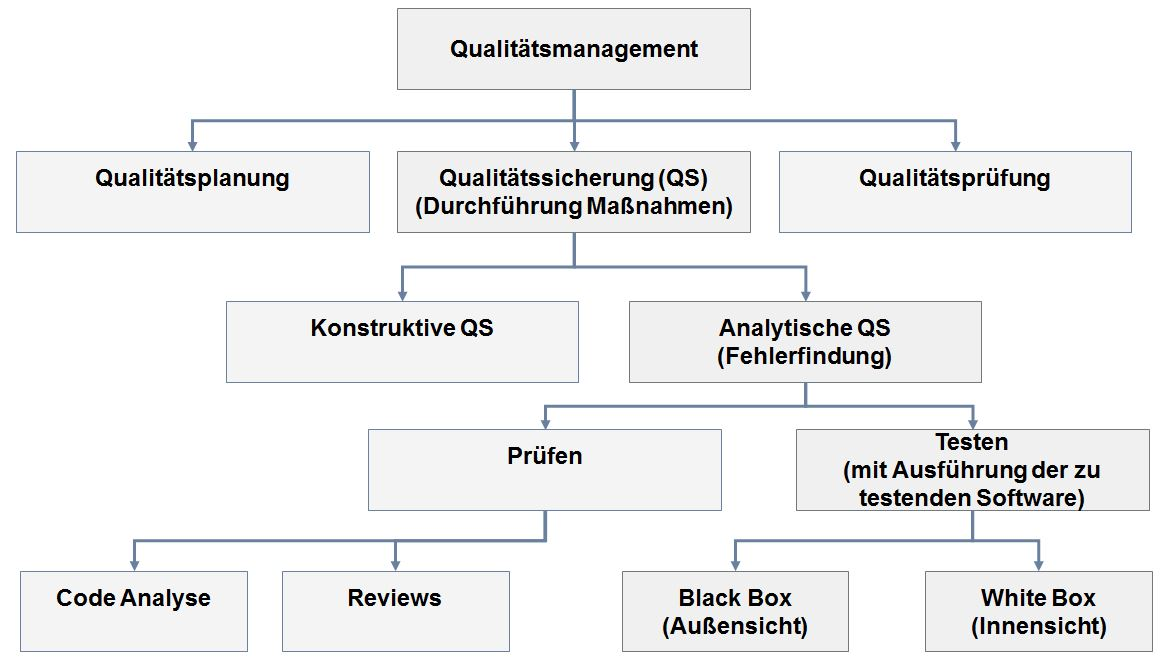
\includegraphics[scale=0.5]{img/qs.jpg}
	\captionof{figure}{\label{abb:sonarqube}Einordnung von SonarQube}
	\vspace{2em}
\end{minipage}




\section{Qualitätsmerkmale von Software}

Um die Qualität von Software bewerten zu können, wurden verschiedene Merkmale festgelegt, welche ausschlaggebend sind. Diese sind nach ISO 25010 genormt. Demnach sind zum Beispiel Faktoren wie Funktionalität, Zuverlässigkeit, Gebrauchstauglichkeit, Sicherheit und Effizienz entscheidend, um die Qualität der Software beurteilen zu können \autocite[Vgl.][]{Merkmale}.

Die Autoren des Buchs \enquote{SonarQube in action} beleuchten dieses Thema ebenfalls sehr umfassend. Sie bewerten die Qualität einer Software nach den sogenannten \enquote{Seven axes of code quality}\autocite[S.13]{SonarInAction}, nach dessen Maßstäben SonarQube geschriebenen Programmcode untersucht. 
Diese Achsen, auch \enquote{Seven Deadly Developer Sins}\autocite[S.13]{SonarInAction} genannt, beinhalten folgende Punkte: Potenzielle Bugs, Programmierrichtlinien, Tests, Duplikationen, Kommentare, Architektur und Design, sowie Komplexität.
Um alle Punkte abdecken zu können, sind die Regeln von SonarQube, anhand derer die Qualität einer Software bemessen wird, auf diese sieben Achsen abgestimmt.



% !TEX root =  master.tex 
\chapter{SonarQube -- Manuel Techert}


\section{Definition von SonarQube}

Die von uns eingesetzte Plattform SonarQube wird hier kurz erklärt.

Die Plattform SonarQube wird in der offiziellen Dokumentation von Ann Campbell folgendermaßen definiert:

\enquote{The SonarQube® platform is an open source quality management platform, dedicated to continuously analyzing and measuring the technical quality of source code, from project portfolio down to the method level, and tracking the introduction of new Bugs, Vulnerabilities, and Code Smells in the Leak Period} \autocite{DefinitionSonarQubeDoc}.

Diese Definition deckt sich mit dem Leitsatz der offiziellen Homepage von SonarQube. Demnach soll SonarQube  die Qualität eines Produktes laufend anhand von Analysen und Kennzahlen protokollieren und etwaige Fehler verfolgbar machen \autocite[Vgl.][]{StartSeiteSonarQube}.


\section{Aufbau und grundlegende technische Voraussetzungen}

\subsection{Die drei Komponenten von SonarQube}

SonarQube ist kein eigenständiges Werkzeug. Es ist eine Plattform, die sich aus drei wesentlichen Komponenten ergibt. 
So besteht diese aus einem SonarQube-Server, der unter anderem für die Verarbeitung und Aufbereitung der Analysen zuständig ist, dessen Ergebnisse sich gespeichert in der zweiten Komponente, der Datenbank, wiederfinden. Zuletzt existiert noch der Scanner, welcher die Analysen übernimmt.


\begin{minipage}{\linewidth}
	\centering
	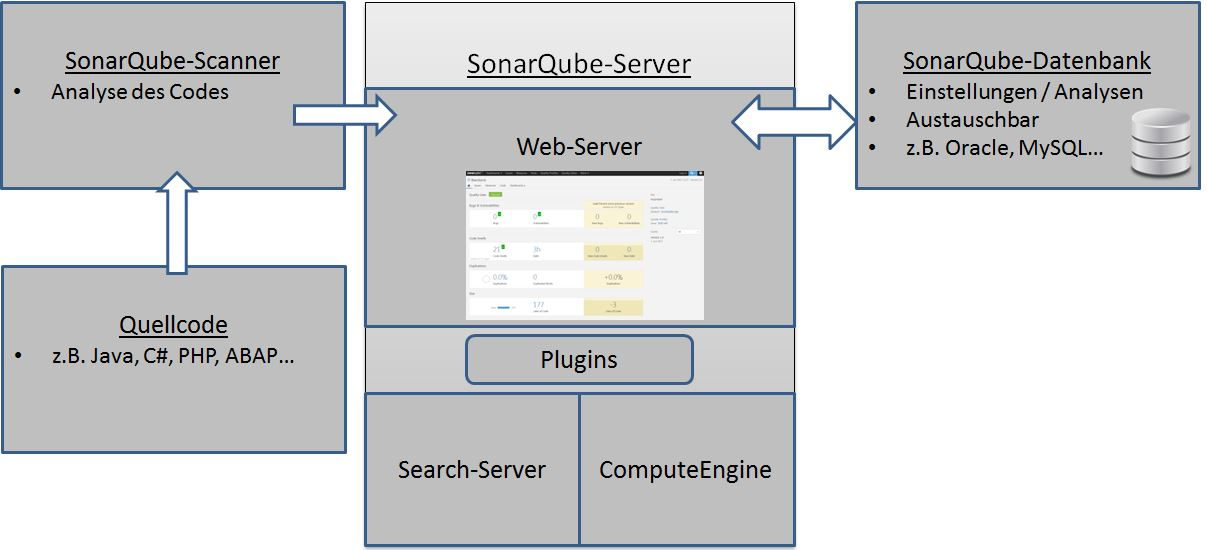
\includegraphics[scale=0.45]{img/SonarAufbau.jpg}
	\captionof{figure}{\label{abb:sonaraufbau}Der Aufbau der Komponenten von SonarQube}
	\vspace{2em}
\end{minipage}

\subsubsection{Der SonarQube-Server}

Der SonarQube-Server, der die Schnittstelle zwischen dem Scanner und der Datenbank darstellt, besteht aus einem \glqq ComputeEngine-Server\grqq{}, dem \glqq Search-Server\grqq{} und zuletzt dem \glqq Web-Server\grqq{} \autocite[Vgl.][]{dotnetpro}.

Wird eine Analyse mithilfe des Scanners durchgeführt, verarbeitet der ComputeEngine-Server diese, um sie im Anschluss in der Datenbank abspeichern zu können.

Sind nun Analysen in der Datenbank hinterlegt, sucht der Search-Server gezielt nach diesen, um sie weiter auf den Web-Server zu reichen.

Im Interface des Web-Servers können schließlich die Ergebnisse der Analysen begutachtet werden. Hier finden sich neben zahlreichen Möglichkeiten, die Ergebnisse zu filtern und zu betrachten, auch diverse Einstellungsmöglichkeiten für SonarQube selbst.

\subsubsection{Die Datenbank}

In der Datenbank werden alle vorgenommenen Einstellungen und Analysen abgespeichert. Eine Eigene ist bei der Installation von SonarQube bereits integriert. Diese ist aber nicht bindend, es können auch Datenbanken wie Microsoft SQL Server, MySQL, Oracle oder PostgreSQL genutzt werden \autocite[Vgl.][]{SonarRequirements}. Da die Menge an analysierten Daten schnell unübersichtlich groß wird, sollte man bei einer ernsthaften Verwendung von SonarQube in jedem Fall die ursprüngliche Datenbank ersetzen.

\subsubsection{Der Scanner}

Der Scanner bildet die Grundlage für Analysen und ist, neben einer lokalen Variante, in verschiedenen Versionen für die unterschiedlichsten Build-Tools verfügbar \autocite[Vgl.][]{VerschScanner}. Diese Tools werden im Softwareentwicklungsprozess oft genutzt, um den Prozess vom Programmieren zum ausführbaren Programm vereinfacht zu verwalten \autocite[Vgl.][]{BuildTools}. Ein Beispiel für solch ein Tool ist Apache Maven, welches auf der offiziellen Seite als \enquote{[...] software project management and comprehension tool.} beschrieben wird \autocite{Maven}.

Ganz gleich in welcher Version, bedient der Scanner sich, um seine Analyse durchführen zu können,  dreierlei Werkzeuge:  \glqq FindBugs\grqq{}, \glqq PMD\grqq{} und \glqq CheckStyle\grqq{} \autocite[Vgl.][]{FindBugsPMDCheckStyle}. Diese Werkzeuge besitzen eigene Metriken, die gegebenen Quelltext oder kompilierten Bytecode hinsichtlich verschiedener Kriterien durchsuchen. 

Der Begriff \enquote{Metrik} ist dabei durch einen IEEE-Standard folgendermaßen normiert:

\enquote{A function whose inputs are software data and whose output is a single numerical value that can be interpreted as the degree to which software possesses a given attribute that affects its quality.}\autocite{IEEE1061-1998}.

Demnach ist eine Metrik eine Funktion, welche aus einem Eingabestrom Ausgabewerte erzeugt, die untereinander vergleichbar sind. Diese Werte sind in der Softwaremetrik Zahlen, deren Höhe Auskunft über die Qualität eines Teils einer Software geben.

Alle Metriken sind in sogenannten Regeln umgesetzt, deren Verstöße, \enquote{Issues} genannt, vermerkt werden.

FindBugs durchsucht den vom Java-Compiler übersetzten Bytecode auf strenge Programmierfehler, wie etwa nicht mögliche Typumwandlungen \autocite[Vgl.][]{FindBugs}. Fehler, die also aufgrund fehlender Kenntnisse oder Flüchtigkeit entstehen, werden von FindBugs entdeckt.

Das nächste Werkzeug, PMD, befasst sich weniger mit Fehlern, sondern eher mit einer Steigerung der Effizienz \autocite[Vgl.][]{PMD}. PMD erkennt somit alles, was optimiert zu einer Leistungssteigerung führt. Beispiele hierfür sind etwa leere Code-Blöcke, die keinen Inhalt haben und damit obsolet sind. Noch ein Beispiel stellen Variablen dar, die zwar initialisiert, aber nie benutzt werden.  Dieses Werkzeug arbeitet, anders als FindBugs nicht auf Bytecode-, sondern auf Quelltextebene.

Zuletzt bedient sich der Scanner noch am Werkzeug CheckStyle. Dieses arbeitet, wie PMD, auf Quelltextebene und prüft die Einhaltung bestimmter Programmier-Konventionen. So sind die hier erkannten \enquote{Fehler} lediglich Vorschläge, die zu einem besseren Stil beitragen und das Programm beispielsweise übersichtlicher machen \autocite[Vgl.][]{CheckStyle}.

Nach dieser Einteilung des Fehlertyps werden Verstöße noch in ihrer Schwere beurteilt. Je nachdem, wie gravierend ein Verstoß wiegt, wird dieser von der Schwere hin absteigend zum Beispiel als \enquote{Blocker} oder \enquote{Critical}, \enquote{Major} oder \enquote{Minor} deklariert \autocite[Vgl.][]{MetricDefinitions}. Auch eine Einstufung als \enquote{Info} ist möglich. Ein Verstoß wird also einmal in seiner Art und darüber hinaus in der Schwere beurteilt.
Alle Stellen im Code, wo eine Optimierung notwendig oder möglich ist, werden durch den Scanner markiert und im Web-Server aufbereitet angezeigt. Die Erkennung läuft bei allen Werkzeugen gleichermaßen ab. Individuell einstellbare Regeln jedes Werkzeugs werden auf ihre Erfüllung hin abgeprüft und Verstöße entsprechend aufgezeigt. Wie in der Einleitung bereits erwähnt, werden alle Regeln bezüglich ihrer Kategorie noch in eine der Sparten Bugs, Code Smells oder Vulnerabilities eingeordnet.


\section{Inbetriebnahme von SonarQube - Überblick}
%und richtige Interpretation der Daten}

SonarQube wird von uns über eine manuelle Installation wie folgt installiert:

Zunächst erfolgt ein Download des SonarQube-Server und eine anschließende Installation. Nach dessen Start kann der Scanner hinzugefügt werden, der nun Projekte analysieren kann. Dies erfolgt über das Terminal in in macOS. Analysierte Projekte werden bei einer nicht an das Internet gebundenen Installation, wie in unserem Fall, unter einer lokalen Webkomponente verfügbar gemacht \autocite[Vgl.][]{GetStarted}.

Ist SonarQube also vollständig installiert, der Server gestartet und wurde bereits eine Analyse durchgeführt, so kann man nun die Ergebnisse in der Webkomponente unter der angegebenen Adresse einsehen. Diese ist im Terminal nach Start des Servers zu sehen. Auf der Startseite des Web-Servers kann nun das untersuchte Projekt angewählt werden (siehe Abbildung 3.2). Die Reiter am oberen Rand, wie zum Beispiel \enquote{Dashboards}, \enquote{Issues} oder \enquote{Quality Gates} stellen allgemeine Optionen der Plattform dar.



\begin{minipage}{\linewidth}
	\centering
	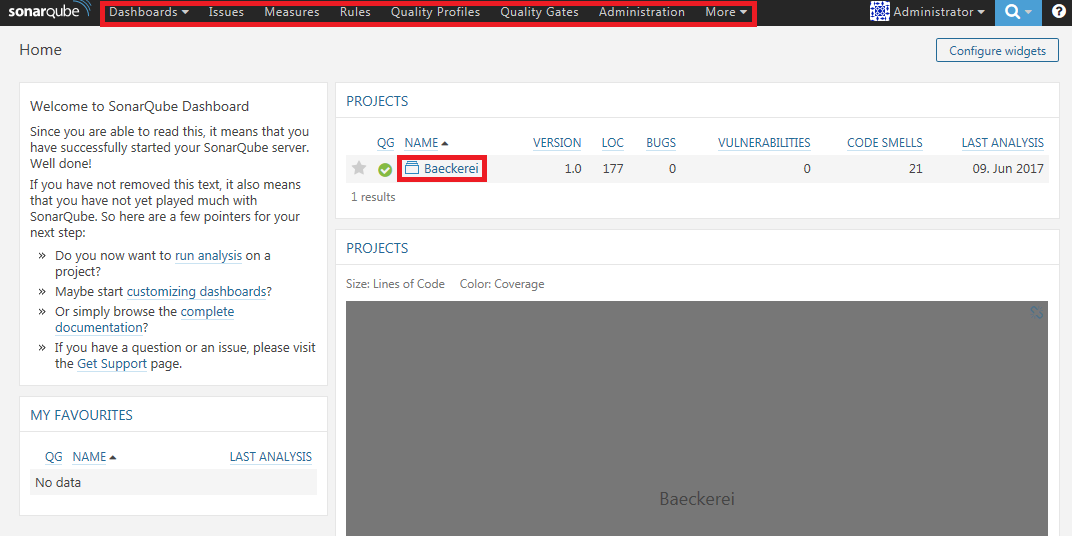
\includegraphics[scale=0.55]{img/StartSeiteSonar.PNG}
	\captionof{figure}{\label{abb:startseitesonar}Die Startseite des Web-Servers}
	\vspace{2em}
\end{minipage}

Sobald ein Projekt ausgewählt wurde, findet sich darunter ein sekundärer Reiter, der explizit das Projekt betrachtet (siehe Abbildung 3.3). Nun befindet man sich auf dem Dashboard eines Projektes. Neben dem erwähnten sekundären Reiter, ist hier eine gute Übersicht über die Merkmale des Projekts gegeben. Unter der Anzahl der \enquote{Bugs und Vulnerabilities} oder den \enquote{Code Smells}, findet man auch Werte für Duplikationen oder die Größe des untersuchten Codes. Auf der rechten Seite sind auch das zugewiesene Quality-Profile oder Quality-Gate aufgeführt.

Mit einem Klick auf \enquote{Issues} kann man alle Regelverstöße einsehen, die das Projekt verursacht hat. Die Sparte \enquote{Measures} präsentiert weitere Qualitätsmerkmale des Projektes, unter anderem \enquote{Reliability}, \enquote{Security} oder \enquote{Maintainability}. Unter \enquote{Code} findet man die Dateistruktur des Projektes, also die Aufteilung in die verschiedenen Packages und Klassen. Ist man mit dem Standard-Dashboard nicht zufrieden, gibt es die Option unter \enquote{Dashboards} seine eigene Übersicht aus zahlreichen Komponenten zusammenzubauen. Der letzte Punkt im Projektreiter, \enquote{Administration} ist nur sichtbar, wenn man als Administrator angemeldet ist und bietet diverse Verwaltungsmöglichkeiten für Speicherzeiträume der Datenbank, Quality-Profiles oder Quality-Gates. Die Rechteverwaltung findet man hier ebenso.



\begin{minipage}{\linewidth}
	\centering
	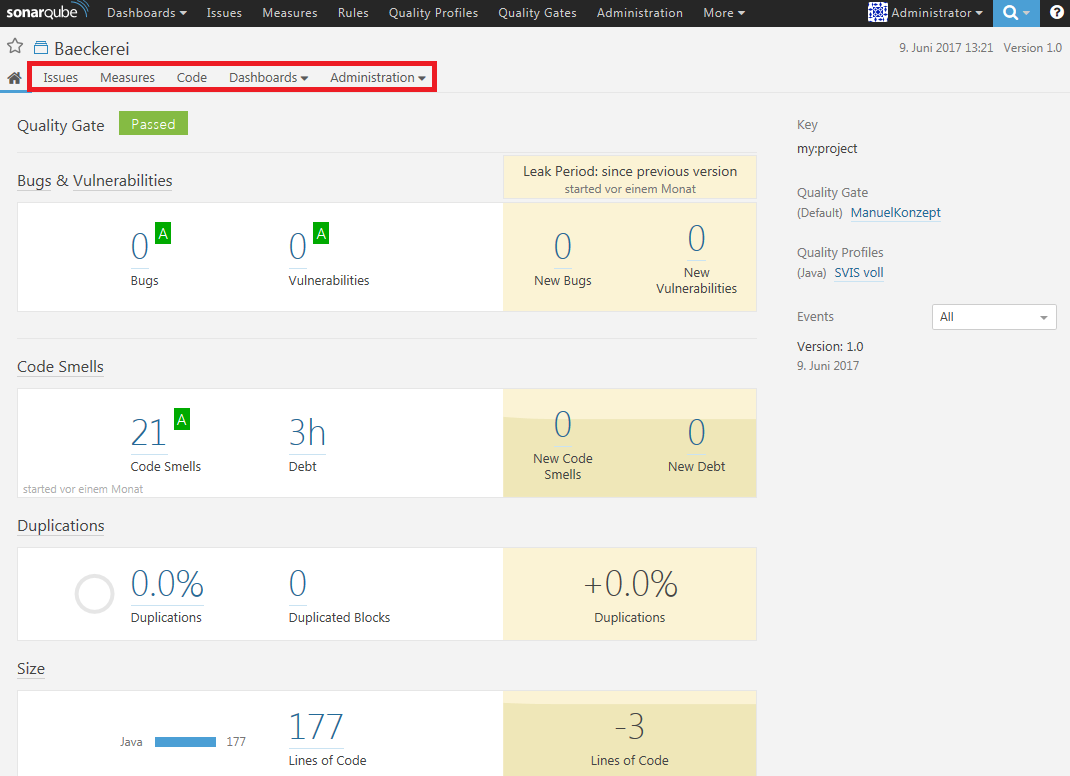
\includegraphics[scale=0.5]{img/StartSeiteSonarNachProjekt.PNG}
	\captionof{figure}{\label{abb:startseitesonarnachprojekt}Das Dashboard}
	\vspace{2em}
\end{minipage}


%Analysen durchführen, durch Filtern ersichtlich machen.
%Fehler verfolgen, evtl. durch Assignments auf einzelne User herunterbrechen.
%Fehler korrigieren, Regeln verstehen
%Fehler kritisch hinterfragen

\subsection{Quality-Profiles erstellen und verwalten}

Die die Analyse des Scanners bestimmenden Regeln können in SonarQube angepasst werden. In einem sogenannten Quality-Profile kann man festlegen, welche Regeln man aus dem Standard-Regelsatz von SonarQube, \enquote{TheSonarWay}, übernehmen möchte \autocite[Vgl.][]{QualityProfile}. So kann man individuell wichtige Regeln aktivieren und nicht benötigte oder störende abschalten.

Die Regeln selbst sind wieder in die drei Kategorien Bugs, Vulnerabilities und Code Smells unterteilt. Bei einem Verstoß gegen eine Regel, wird dieser entsprechend mit seiner zugehörigen Kategorie angezeigt. Wird also ein Verstoß gegen eine Regel aus dem Bereich \enquote{Bugs} erkannt, wird im Web-Server der Verstoß ebenso als Bug deklariert. Bei einigen Regeln kann man die darin enthaltenen Kriterien mit verschiedenen Parametern auf die Empfindlichkeit anpassen.
Jedem Projekt, also jeder Ansammlung von Klassen aus einer beliebig unterstützten Programmiersprache kann zu jeder Zeit genau ein Quality-Profile zur Nutzung zugewiesen werden, nach dessen Regeln es untersucht wird. Zusätzlich ist ein Standard-Quality-Profile festgelegt, das auch dann greift, wenn die Verbindung zum Server fehlt und damit das zu nutzende Profile nicht geladen werden kann \autocite[Vgl.][]{QualityProfile}. Beim Erstellen neuer Quality-Profiles ist es auch möglich, Regeln von anderen Profilen zu erben, um sich so das aufwendige Einfügen gleicher Regeln zu ersparen. Ebenso können Quality-Profiles heruntergeladen und wiederhergestellt werden. Dies geschieht über die Optionen \enquote{Restore} und \enquote{Backup} unter der Kategorie \enquote{Quality-Profiles}. Gespeichert werden die Profile im .xml-Format. Somit lassen sich präferierte Regeln auch über mehrere Versionen hinweg sichern und wiederherstellen \autocite[Vgl.][]{QualityProfile}.
Wir haben aus dem großen Regelsatz die für uns wichtigsten Regeln ausgewählt und diese in einem Quality-Profile namens \enquote{fallstudie} gesammelt und danach aktiviert.

\subsection{Quality-Gate anpassen}

Um nun die Qualität der eigenen Software besser verfolgen zu können, kann man \enquote{Quality-Gates} auf dem SonarQube-Server einrichten, die als metaphorisches Prüftor dienen, welches die Software passieren muss \autocite[Vgl.][]{QualityGate}. Die Anwendung passiert dieses Tor nur dann, wenn vorher gesetzte Anforderungen erfüllt sind. Ist dies nicht der Fall, kann die Software nicht passieren.

Unter anderem kann bei der Einrichtung eines solchen Gates festgelegt werden, wie schwer verschiedene Arten von Fehlern wiegen oder wie viele Fälle eine \enquote{case} -Anweisung in der Programmiersprache Java höchstens haben darf. Diese Anforderungen sind alle vollständig frei setzbar und dienen daher dazu, die eigenen Qualitätsanforderungen an die Software besser umsetzen zu können. Noch dazu wird unterschieden, ob ein gewisses Kriterium zu jeder Zeit erfüllt werden muss oder nur über einen längeren Zeitraum gegeben sein muss \autocite[Vgl.][]{QualityGate}. 
Als kleines Beispiel kann eingestellt werden, dass die Software zu jeder Zeit nur fünf Bugs haben darf. Führt man nun eine Analyse durch und betrachtet die Ergebnisse, wird zugleich ausgegeben, ob die Software den Anforderungen des Quality-Gates gerecht geworden ist und somit passieren kann oder ob hier noch nachgearbeitet werden muss. Bei vier Bugs zu einem beliebigen Zeitpunkt würde das Gate passiert werden, ab sechs nicht mehr.

Generell ist immer eine Bedingung in Kombination mit einem Operator, wie z.B. \enquote{größer}, \enquote{kleiner} oder \enquote{gleich} wählbar. Dazu kommen noch zwei Richtwerte, die gesetzt werden müssen, um festzulegen, ab welchem Wert, in Verbindung mit dem Operator, ein Error oder eine Warnung erzeugt wird. Analog zu den Quality-Profiles können die Einstellungen zum Quality-Gate im Webinterface vorgenommen werden. Auch das als Standard zu nutzende Quality-Gate muss festgelegt werden, da ansonsten wieder auf das von der Installation mitgebrachte Quality-Gate zugegriffen wird.

Da uns primär das Finden von Fehlerquellen wichtig war, haben wir die Einstellungen des Quality-Gates zunächst auf den Standard-Einstellungen gelassen, die bestimmten, das keine neuen, schweren Issues hinzukommen dürfen. So haben wir laufend versucht, von vorneherein Fehlerquellen gar nicht erst entstehen zu lassen.


\begin{minipage}{\linewidth}
	\centering
	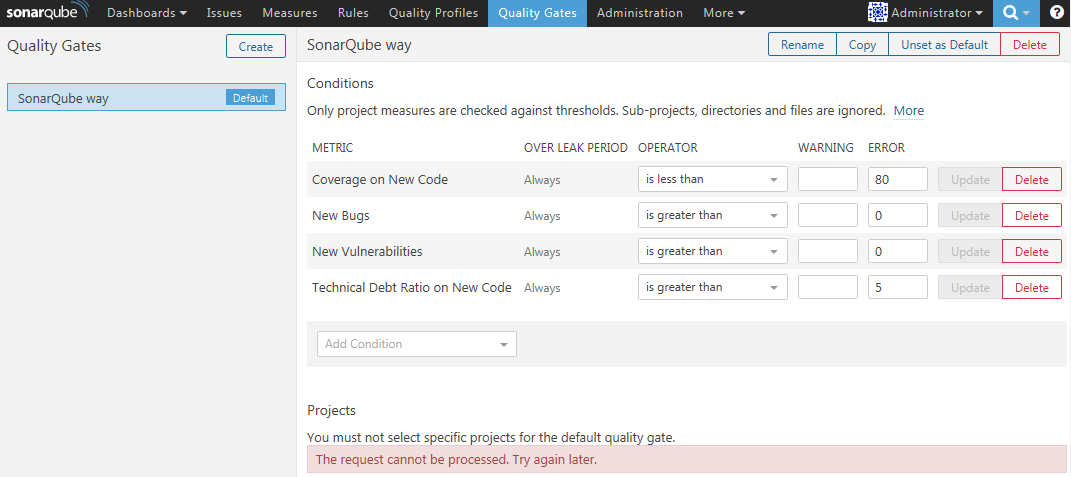
\includegraphics[scale=0.55]{img/QualityGate.PNG}
	\captionof{figure}{\label{abb:qualitygate}Beispielkonfiguration eines Quality-Gates}
	\vspace{2em}
\end{minipage}



% !TEX root =  master.tex 
\chapter{Bereinigung von Fehlern -- Manuel Techert}

Gegen Ende des Projekts wollen wir die Qualität unseres Projektes noch einmal erhöhen und etwaigen Fehlern vorbeugen.

Dazu nutzen wir die Plattform SonarQube, die uns bei einem Verstoß gegen unsere definierten Regeln mitteilt, wo nachgebssert werden sollte. 

Um einen aktuellen Stand unsere Regelverstöße zu haben, führe ich eine Analyse mit dem Scanner von SonarQube zu, dessen Ergebnisse im Web-Server abgelegt werden (siehe nachfolgende Abbildung).
\\

\begin{minipage}{\linewidth}
	\centering 
	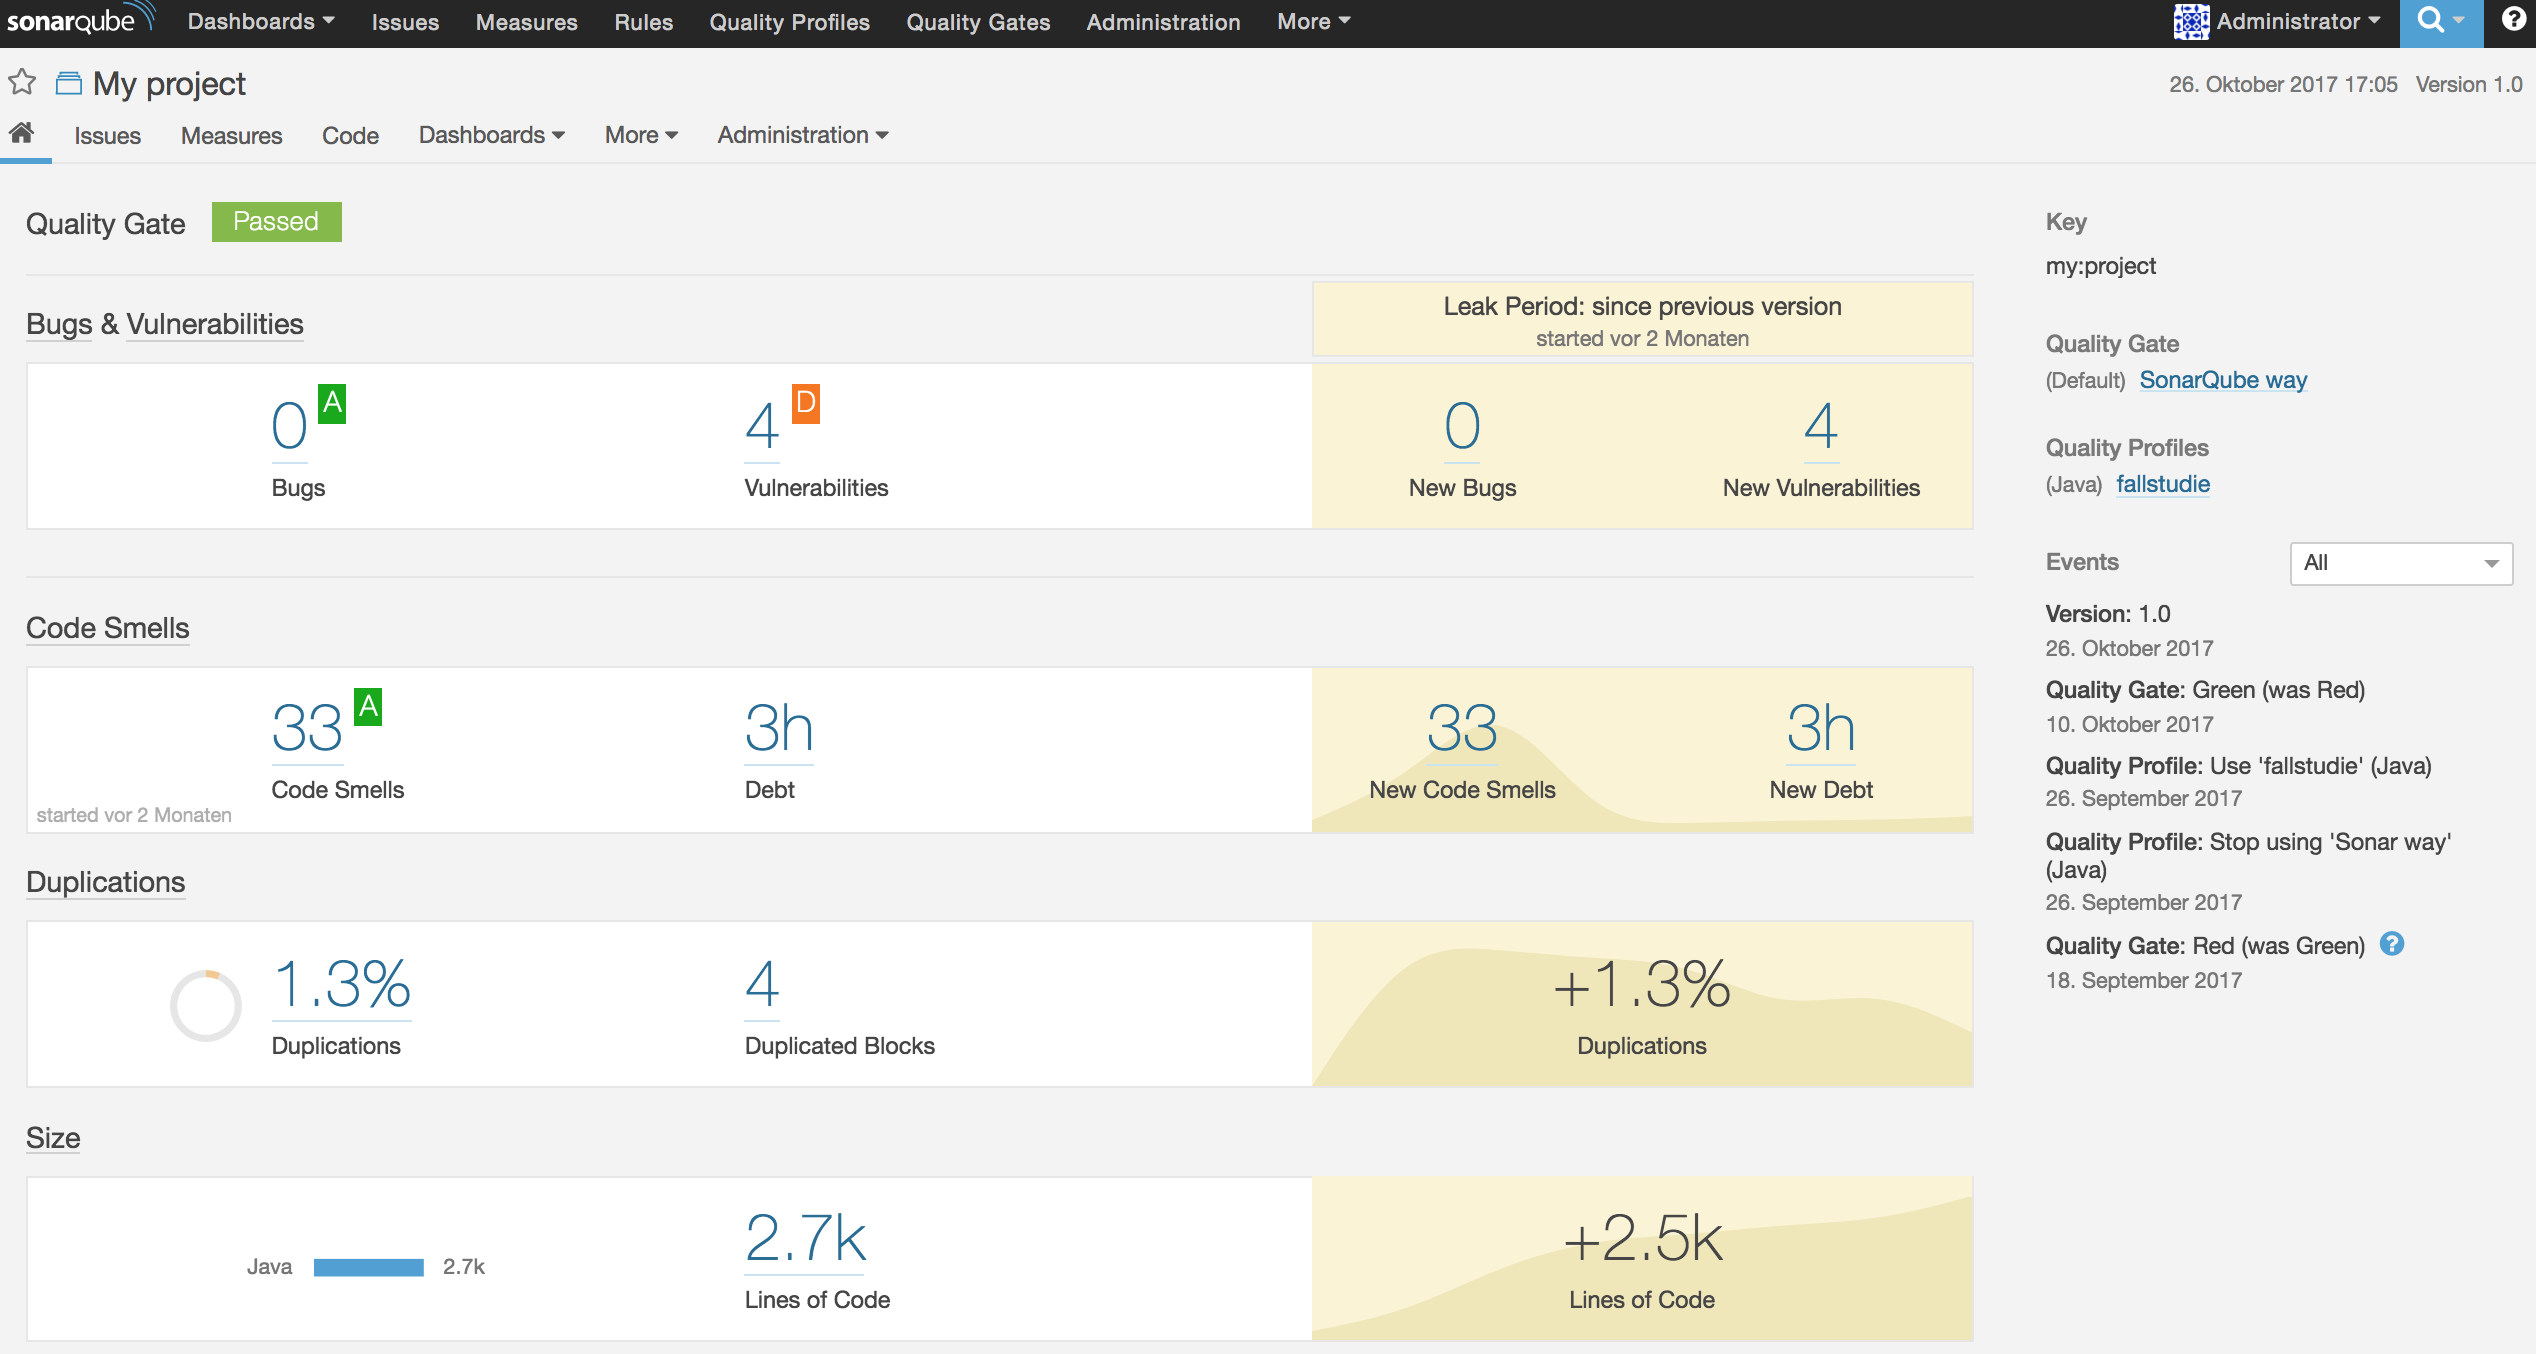
\includegraphics[scale=0.35]{img/startSonar}
	\captionof{figure}{\label{abb:startsonar}Die Startseite des SonarQube-Servers.}
	\vspace{2em}
\end{minipage}

Bei Einsicht der Ergebnisse sehen wir, dass wir an einigen Stellen Strings mit einem doppelten Gleichzeichen statt dem equals-Ausdruck verglichen haben. Da SonarQube die Verstöße auf die einzelnen Klassen verfolgbar macht, gelingt es uns in kurzer Zeit die vorhandenen Verstöße zu entfernen.

\begin{minipage}{\linewidth}
	\centering 
	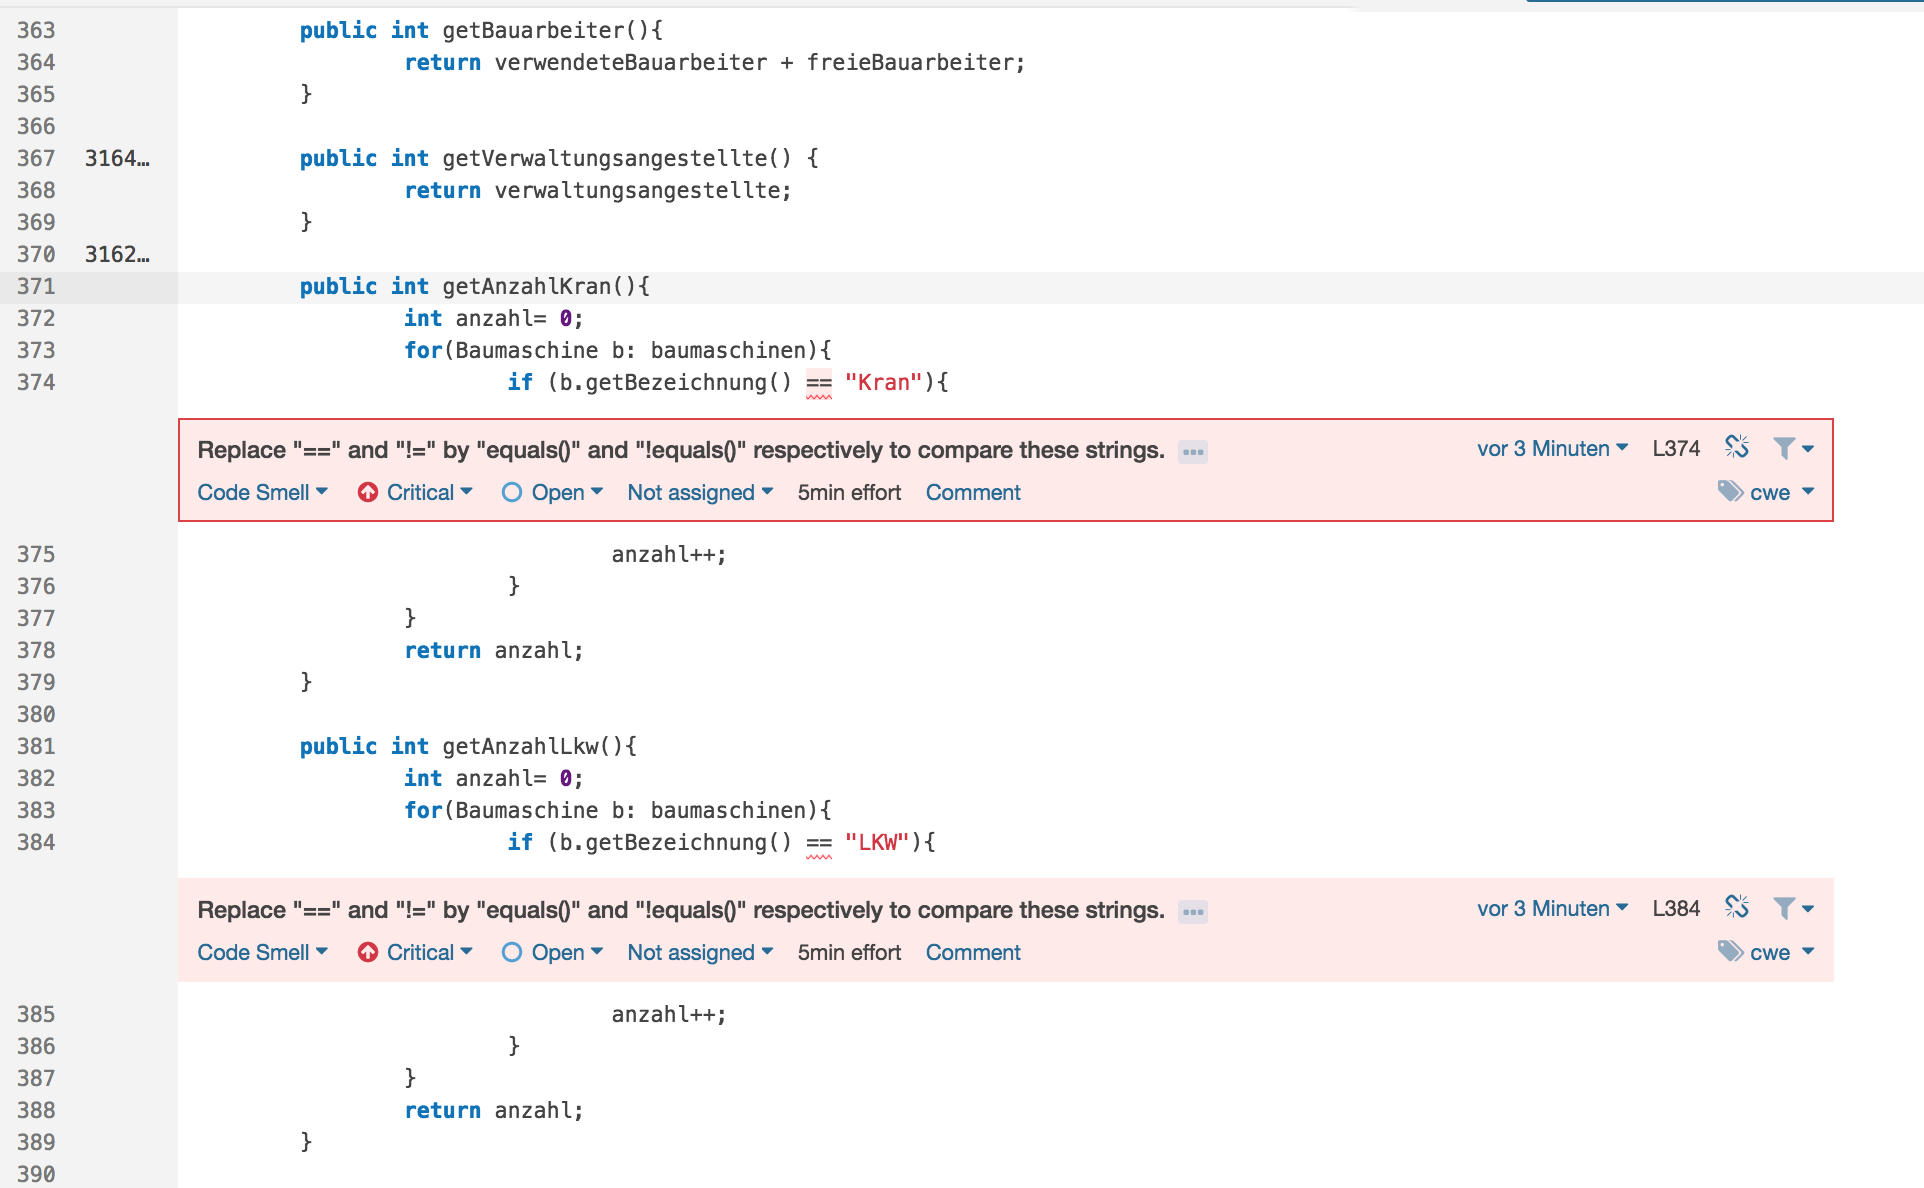
\includegraphics[scale=0.45]{img/fehlerSonar}
	\captionof{figure}{\label{abb:fehlersonar}Sonar entdeckt das Verwenden eines doppelten Gleichzeichens statt eines equals-Ausdruck.}
	\vspace{2em}
\end{minipage}


% !TEX root =  master.tex 
\chapter{Fazit und Reflexion des Projekts}














\clearpage % Römische Seitennummerierung
\pagenumbering{roman}\setcounter{page}{7} % ACHTUNG DIESE Zahl muss manuell eingegeben werden 

%	Literaturverzeichnis
\ihead{} % Neue Header-Definition
\printbibliography[title=Literaturverzeichnis]
%\nocite{*} % DANIEL Fügt alles dem Literaturverzeichnis hinzu, egal ob zitiert oder nicht
\cleardoublepage


% Der Anhang beginnt hier - jedes Kapitel wird alphabetisch aufgezählt. (Anhang A, B usw.)
\appendix
\ihead{\appendixname~\thechapter} % Neue Header-Definition

% appendix.tex einziehen
%% !TEX root =  master.tex

\chapter{Anhang}




% Ehrenwörtliche Erklärung ewerkl.tex einziehen
% !TEX root =  master.tex

\clearpage
\chapter*{Ehrenwörtliche Erklärung}

% Wird die folgende Zeile auskommentiert, erscheint die ehrenwörtliche
% Erklärung nicht im Inhaltsverzeichnis.

\addcontentsline{toc}{chapter}{Ehrenwörtliche Erklärung}


Wir, Daniel Pies, Thomas Pötz und Manuel Techert, versichern hiermit, dass wir die hier vorliegende Gruppenarbeit mit dem Thema:
 
\begin{quote}
	\textit{Fallstudie \DerTitelDerArbeit}
\end{quote}

selbstständig verfasst und keine anderen als die angegebenen Quellen und Hilfsmittel benutzt haben. Wir versichern zudem, dass die eingereichte elektronische Fassung mit der gedruckten Fassung übereinstimmt. Wir sind uns bewusst, dass eine falsche Erklärung rechtliche Folgen haben wird.

\vspace{2.2cm}
Mannheim, den 13. November 2017 \hfill Daniel Pies

\vspace{2.2cm}
Mannheim, den 13. November 2017 \hfill Thomas Pötz

\vspace{2.2cm}
Mannheim, den 13. November 2017 \hfill Manuel Techert


%\renewcommand{\baselinestretch}{1}\normalsize % um Zeilenabstand am Ende zurück zusetzen

\end{document}
